\documentclass[11pt,letterpaper]{article}

%=====================================================
% PREÁMBULO: PAQUETES Y CONFIGURACIÓN FORMAL
%=====================================================
\usepackage[utf8]{inputenc}
\usepackage[spanish, es-tabla]{babel}
\usepackage{geometry}
\geometry{top=2.5cm, bottom=2.5cm, left=3cm, right=3.5cm} % Margen estándar fijado

\usepackage{booktabs}   % Líneas profesionales para tablas
\usepackage{array}      % Control avanzado de columnas
\usepackage{tabularx}   % Tablas con ancho ajustable
\usepackage{float}      % Control estricto de posición [H]
\usepackage{enumitem}   % Personalización avanzada de listas
\usepackage{titlesec}   % Control de formato de títulos
\usepackage{graphicx}   % Inclusión de imágenes
\usepackage{caption}    % Personalización de leyendas

% Configuración de leyendas
\captionsetup[figure]{labelfont=bf, textfont=normalfont}
\captionsetup[table]{labelfont=bf, textfont=normalfont}

% Formato de títulos de sección (Mayúsculas y tamaños según tu requerimiento)
\titleformat{\section}{\normalfont\fontsize{14}{16}\bfseries}{\thesection.}{1em}{\MakeUppercase}
\titlespacing*{\section}{0pt}{2.5ex plus 1ex minus .2ex}{1.5ex plus .2ex}

\titleformat{\subsection}{\normalfont\fontsize{12}{14}\bfseries}{\thesubsection.}{1em}{\MakeUppercase}
\titlespacing*{\subsection}{0pt}{1.8em plus 0.4em minus 0.2em}{0.8em plus 0.2em}

\titleformat{\subsubsection}{\normalfont\normalsize\bfseries}{\thesubsubsection.}{0.5em}{}

% Ajuste de las listas estilo académico
\setlist[itemize]{topsep=2pt, itemsep=1pt, parsep=0pt, leftmargin=1.5em}
\setlist[enumerate]{topsep=2pt, itemsep=1pt, parsep=0pt, leftmargin=1.5em}

\setlength{\parindent}{1.25cm}     % Sangría formal
\setlength{\parskip}{1em}          % Espaciado entre párrafos

% MATEMÁTICAS Y UNIDADES
\usepackage{amsmath}
\usepackage{siunitx}
\sisetup{
  locale=FR,
  group-separator={.}
}

% ==========================================
% CONFIGURACIÓN DE TABLA DE CONTENIDO Y FORMATO
% ==========================================
\usepackage{tocloft}
\renewcommand{\cftsecleader}{\cftdotfill{\cftdotsep}}
\usepackage{float}

% Carga de paquetes para tablas y unidades
\usepackage{booktabs}
\usepackage{array}
\usepackage{makecell}
\usepackage{siunitx}

% Configuración a prueba de fallas para Chile (Decimales con coma y miles con punto)
\sisetup{
  output-decimal-marker = {,},  % El PDF resultante mostrará coma para decimales
  group-separator = {.},         % El PDF agrupará miles usando puntos (ej: 14.514)
  group-minimum-digits = 4       % Agrupa miles a partir de 4 dígitos
}

% ENCABEZADOS Y PIE DE PÁGINA
\usepackage{fancyhdr}
\pagestyle{fancy}
\fancyhf{}

\setlength{\headheight}{18pt}
\renewcommand{\headrulewidth}{0.5pt}

\fancyhead[L]{%
\raisebox{-0.25\height}{
\includegraphics[height=0.6cm]{Logo Construcción Uach.jpg}}%
\hspace{0.3cm}
\fontsize{9}{11}\selectfont Álvaro Flores V.%
}
\fancyhead[R]{\fontsize{9}{11}\selectfont IOCC297 -- Trabajo de Título}
\fancyfoot[R]{\thepage}

% LISTINGS (CONFIGURACIÓN DE CÓDIGO)
\usepackage{listings}
\usepackage{xcolor} 

\definecolor{codigoFondo}{rgb}{0.95, 0.95, 0.92}
\definecolor{codigoGris}{rgb}{0.5, 0.5, 0.5}
\definecolor{codigoVerde}{rgb}{0, 0.6, 0}
\definecolor{codigoAzul}{rgb}{0, 0, 1}
\definecolor{codigoMagenta}{rgb}{0.58, 0, 0.82}

\lstset{
    backgroundcolor=\color{codigoFondo},
    basicstyle=\ttfamily\footnotesize,
    breakatwhitespace=false,
    breaklines=true,
    captionpos=b,
    commentstyle=\color{codigoVerde},
    keepspaces=true,
    keywordstyle=\color{codigoAzul},
    numbers=left,
    numbersep=5pt,
    numberstyle=\tiny\color{codigoGris},
    showspaces=false,
    showstringspaces=false,
    showtabs=false,
    stringstyle=\color{codigoMagenta},
    tabsize=4,
    inputencoding=utf8,
    extendedchars=true,
    literate=
      {á}{{\'a}}1 {é}{{\'e}}1 {í}{{\'i}}1 {ó}{{\'o}}1 {ú}{{\'u}}1
      {Á}{{\'A}}1 {É}{{\'E}}1 {Í}{{\'I}}1 {Ó}{{\'O}}1 {Ú}{{\'U}}1
      {ñ}{{\~n}}1 {Ñ}{{\~N}}1 {¿}{{\textquestiondown}}1 {¡}{{\textexclamdown}}1
}

% BIBLIOGRAFÍA
\usepackage{csquotes}
\usepackage[
  backend=biber,
  style=authoryear,
  sorting=nyt,
  maxcitenames=2,
  uniquelist=false,
  giveninits=true,
  doi=false,
  isbn=false,
  eprint=false,
  url=true
]{biblatex}

\addbibresource{ReferenciasSUS.bib}
\DeclareDelimFormat{nameyeardelim}{\addcomma\space}

\usepackage[titletoc]{appendix}
\setlength{\bibitemsep}{1em}

% HIPERVÍNCULOS (SIEMPRE AL FINAL DEL PREÁMBULO)
\usepackage[
  unicode=true,
  hidelinks,
  pdfencoding=auto
]{hyperref}

%=====================================================
% INICIO DEL DOCUMENTO
%=====================================================
\begin{document} 

% --- PORTADA ---
\begin{titlepage}
    \begin{center}
        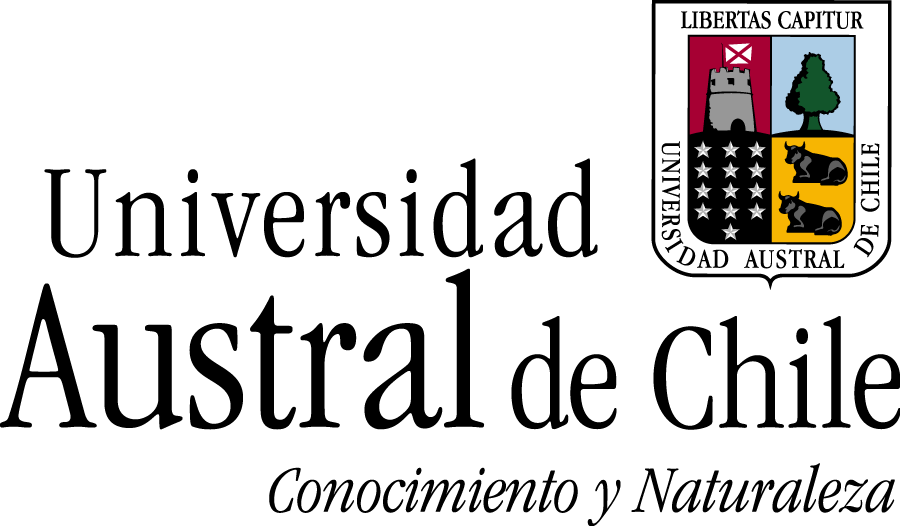
\includegraphics[width=0.4\textwidth]{UACh-color-negro.png} \\
        \textbf{\large Facultad de Ciencias de la Ingeniería} \\
        \vspace{0.5em} 
        \textbf{Escuela de Ingeniería en Construcción}
        
        \vspace{6em} 
        
        {\huge \textbf{TRABAJO DE TITULO} \par} 
        \vspace{1em}
        {\large \MakeUppercase{\textbf{Caracterización del Asfalto Poroso por Métodos Acústicos}} \par} 
        \vspace{8em} 
    \end{center}

    \begin{flushright}
        \renewcommand{\arraystretch}{1.3}       
        \begin{tabular}{rl}
            \textbf{Asignatura:} & IOCC297 -- Trabajo de Título\\
            \textbf{Carrera:}    & Ingeniería en Construcción \\
            \textbf{Docente:}    & Ph.D. Uwe Muhlich Muhlich\\
            \textbf{Alumno:}     & Álvaro Flores Varas \\
            \textbf{Fecha:}      & 28/11/2026
        \end{tabular}
    \end{flushright}

    \vfill 

    \begin{center}
        II semestre de 2026, Valdivia, Chile.
    \end{center}
\end{titlepage}

% --- ÍNDICE ---
\newpage
\pagenumbering{gobble} 
\thispagestyle{empty}
\tableofcontents
\clearpage             

% --- CUERPO DEL INFORME ---
\pagenumbering{arabic} 
\setcounter{page}{4}   
\pagestyle{fancy}      

\part{Marco Teórico}

\section{Fundamentos Físico-Matemáticos de la Acústica}\label{sec:marco-teorico}

\subsection{Ecuación de Continuidad (Conservación de Masa)}

En el desarrollo de la formulación analítica de la acústica, es fundamental partir de los principios de conservación de los medios continuos. 

\begin{itemize}
    \item \textbf{Magnitud $q$:} Representa cualquier cantidad física extensiva que puede fluir o moverse en el medio (por ejemplo: masa, energía, carga eléctrica, impulso, número de moléculas, entre otros).
    \item \textbf{Densidad de volumen $\rho$:} Corresponde a la concentración de la cantidad $q$ por unidad de volumen ($q$ por unidad de volumen).
    \item \textbf{Flujo $\mathbf{J}$:} El flujo de la cantidad $q$ es un campo vectorial que describe cuánta cantidad cruza una determinada área por unidad de tiempo. Si existe un campo de velocidad $\mathbf{v}$ que describe el flujo en cuestión, y toda la cantidad $q$ en un punto $\mathbf{x}$ se mueve con dicha velocidad $\mathbf{v}(\mathbf{x})$, entonces el flujo se expresa como la densidad multiplicada por el campo de velocidad:
    \begin{equation}
        \mathbf{J} = \rho q \mathbf{v}
    \end{equation}
    Por ejemplo, en el caso del agua, correspondería al caudal (la densidad del agua en cada punto $\mathbf{x}$ multiplicada por la velocidad del fluido en cada punto $\mathbf{x}$).
    \item \textbf{Dimensión del flujo:} Cantidad de $q$ que fluye por unidad de tiempo a través de una unidad de área.
    \item \textbf{Integral de superficie:} Si se considera una superficie imaginaria cerrada $S$ que delimita un volumen $V$, la integral de superficie del flujo sobre $S$ representa la cantidad total de $q$ que atraviesa la superficie $S$ por unidad de tiempo:
    \begin{equation}
        \Phi = \oint_S \mathbf{J} \cdot d\mathbf{S}
    \end{equation}
    \item \textbf{Balance de variación en una región:} La cantidad de $q$ contenida en una región aumenta cuando entra $q$ adicional a través de su superficie y disminuye cuando sale. Asimismo, la cantidad de $q$ en una región aumenta cuando se crea nuevo $q$ dentro de ella (fuentes) y disminuye cuando se destruye (sumideros).
    \item \textbf{Tasa de aumento de $q$ en un volumen $V$:} Planteando el balance integral, la derivada temporal de la cantidad acumulada más el flujo neto saliente a través de la superficie es igual a la suma de las tasas netas de generación interna:
    \begin{equation}
        \frac{\partial}{\partial t} \int_V \rho q \, dV + \oint_S \mathbf{J} \cdot d\mathbf{S} = \int_V s \, dV
    \end{equation}
    donde $s$ representa la tasa neta a la que $q$ se genera dentro del volumen $V$ por unidad de tiempo y volumen. En consecuencia, si la derivada parcial o la tasa de acumulación es mayor que cero, $q$ se está generando; si es menor que cero, $q$ se está destruyendo.
\end{itemize}

\subsection{Campo de Velocidades y Balance de Flujo}

\begin{itemize}
    \item \textbf{Campo de velocidad $\mathbf{v}(x,y,z,t)$:} Indica que en cada rincón del espacio y en cada instante de tiempo existe una velocidad distinta.
    \item \textbf{Integral de superficie $\oint_S \mathbf{J} \cdot d\mathbf{S}$:} La integral sobre una superficie cerrada $S$ mide el \textbf{flujo neto} que sale de ese volumen por unidad de tiempo, donde dicho volumen es una región del espacio encerrada por la superficie.
    \item \textbf{Cantidad total $Q$ dentro del volumen $V$:} Si $\rho_q$ es la cantidad por unidad de volumen, para conocer la cantidad acumulada dentro de todo el volumen $V$ se debe sumar la densidad $\rho_q$ en infinitos pequeños cubitos de volumen $dV$:
    \begin{equation}
        Q(t) = \int_V \rho_q \, dV
    \end{equation}
    \item \textbf{Tasa de cambio temporal:} ¿Cómo cambia esa cantidad total a medida que pasa el tiempo? Está dada por la derivada temporal de la integral:
    \begin{equation}
        \frac{\partial}{\partial t} \int_V \rho_q \, dV
    \end{equation}
    Esto describe cómo cambia la cantidad total acumulada dentro de todo el volumen $V$ con el transcurso del tiempo.
    \item \textbf{Vector de área infinitesimal $d\mathbf{S}$:} Al considerar un pequeño trozo de la superficie $S$, se define el vector de área infinitesimal $d\mathbf{S}$, cuya magnitud es el área y cuya dirección apunta siempre hacia afuera del volumen.
    \item \textbf{Producto escalar $\mathbf{J} \cdot d\mathbf{S}$:} Nos indica cuánta cantidad atraviesa ese pequeño trozo de área por unidad de tiempo (convirtiéndose en positivo si sale del volumen y negativo si entra).
    \item \textbf{Flujo neto saliente:} Se obtiene integrando el producto escalar sobre toda la superficie cerrada $S$:
    \begin{equation}
        \text{Flujo Neto Saliente} = \oint_S \mathbf{J} \cdot d\mathbf{S}
    \end{equation}
\end{itemize}

\subsection{Generación Total y Teorema de la Divergencia de Gauss}

\begin{itemize}
    \item \textbf{Generación interna ($\sigma$):} Corresponde a la generación por unidad de volumen y por unidad de tiempo. Es decir, nos indica cuánta cantidad se genera localmente. Para calcular cuánta cantidad se genera en todo el volumen $V$, se integra sobre dicho volumen:
    \begin{equation}
        \text{Generación Total} = \int_V \sigma \, dV
    \end{equation}
    
    \item \textbf{Ecuación de balance general:} Juntando la tasa de variación temporal, el flujo neto saliente a través de la superficie y la generación total, se plantea la relación de conservación:
    \begin{equation}
        \frac{\partial}{\partial t} \int_V \rho \, dV = -\oint_S \mathbf{J} \cdot d\mathbf{S} + \int_V \sigma \, dV
    \end{equation}
    Reordenando los términos para expresar la generación total:
    \begin{equation}
        \int_V \sigma \, dV = \frac{\partial}{\partial t} \int_V \rho \, dV + \oint_S \mathbf{J} \cdot d\mathbf{S}
    \end{equation}

    \item \textbf{Transformación a integral de volumen (Teorema de la Divergencia):} Para que toda la expresión quede en función del volumen, es necesario transformar la integral de superficie cerrada en una integral de volumen mediante el \textbf{Teorema de la Divergencia de Gauss}.
    
    \item \textbf{Interpretación física de la divergencia:} Si se divide el gran volumen $V$ en millones de pequeños cubitos pegados entre sí, estos cubitos comparten las paredes internas. El flujo $\mathbf{J}$ que sale de un cubito $A$ entra exactamente en el cubito vecino $B$, de modo que todas las caras internas se cancelan y solo sobrevive la frontera externa $S$. 
    
    \item \textbf{Definición de divergencia ($\nabla \cdot \mathbf{J}$):} Representa cuánta cantidad ``nace'' o ``brota'' neta desde un punto infinitesimal hacia afuera en todas las direcciones. Por definición, el flujo total a través de la superficie de cualquier volumen es exactamente igual a la integral de la divergencia en el interior de ese volumen:
    \begin{equation}
        \oint_S \mathbf{J} \cdot d\mathbf{S} = \int_V (\nabla \cdot \mathbf{J}) \, dV
    \end{equation}

    \item \textbf{Formulación matemática de la divergencia en un punto:} Se define formalmente tomando el límite cuando el volumen infinitesimal $V_i$ tiende a cero:
    \begin{equation}
        (\nabla \cdot \mathbf{J})_i = \lim_{V_i \to 0} \frac{1}{V_i} \oint_{S_i} \mathbf{J} \cdot d\mathbf{S}
    \end{equation}
    Este límite obliga a la pequeña burbuja o volumen a encogerse hasta el colapso. Para un volumen pequeño, la integral de superficie se aproxima como:
    \begin{equation}
        \oint_{S_i} \mathbf{J} \cdot d\mathbf{S} \approx (\nabla \cdot \mathbf{J})_i \, V_i
    \end{equation}

    \item \textbf{Suma de las cajitas infinitesimales:} Para un volumen de tamaño cualquiera $V$ compuesto por $N$ cajitas $V_i$ contiguas, el flujo neto total es la suma de los flujos que salen de cada cajita:
    \begin{equation}
        \oint_S \mathbf{J} \cdot d\mathbf{S} = \sum_{i=1}^{N} \oint_{S_i} \mathbf{J} \cdot d\mathbf{S}
    \end{equation}
    Dado que las caras internas se cancelan mutuamente, al tomar el límite cuando los volúmenes tienden a cero ($V_i \to 0$) y el número de elementos tiende a infinito ($N \to \infty$), la sumatoria discreta se convierte en una integral continua de volumen:
    \begin{equation}
        \lim_{\substack{V_i \to 0 \\ N \to \infty}} \sum_{i=1}^{N} (\nabla \cdot \mathbf{J})_i \, V_i = \int_V (\nabla \cdot \mathbf{J}) \, dV
    \end{equation}
    Llegando finalmente a la identidad fundamental del Teorema de la Divergencia:
    \begin{equation}
        \oint_S \mathbf{J} \cdot d\mathbf{S} = \int_V (\nabla \cdot \mathbf{J}) \, dV
    \end{equation}
\end{itemize}

\subsection{Ecuación de Conservación Diferencial y Ley de Continuidad de la Masa}

A partir del desarrollo anterior basado en sumas de Riemann y la aplicación del Teorema de la Divergencia de Gauss, se tenía la relación para la generación total en el volumen $V$:
\begin{equation}
    \int_V \sigma \, dV = \frac{\partial}{\partial t} \int_V \rho \, dV + \oint_S \mathbf{J} \cdot d\mathbf{S}
\end{equation}

Sustituyendo la integral de superficie por su equivalente en integral de volumen mediante la divergencia ($\nabla \cdot \mathbf{J}$):
\begin{equation}
    \int_V \sigma \, dV = \frac{\partial}{\partial t} \int_V \rho \, dV + \int_V (\nabla \cdot \mathbf{J}) \, dV
\end{equation}

Ingresando la derivada temporal dentro de la integral (asumiendo condiciones de regularidad adecuadas para pasar del operador discreto al continuo):
\begin{equation}
    \int_V \sigma \, dV = \int_V \frac{\partial \rho}{\partial t} \, dV + \int_V (\nabla \cdot \mathbf{J}) \, dV
\end{equation}

Reorganizando todos los términos en una sola integral de volumen igualada a cero:
\begin{equation}
    \int_V \left( \frac{\partial \rho}{\partial t} + \nabla \cdot \mathbf{J} - \sigma \right) dV = 0
\end{equation}

Dado que esta expresión debe cumplirse de manera estricta para \textbf{cualquier volumen arbitrario $V$} del espacio, el integrando mismo debe ser idénticamente cero en cada punto del dominio:
\begin{equation}
    \frac{\partial \rho}{\partial t} + \nabla \cdot \mathbf{J} - \sigma = 0
\end{equation}

Despejando, se obtiene la forma diferencial general de la ecuación de conservación:
\begin{equation}
    \frac{\partial \rho}{\partial t} + \nabla \cdot \mathbf{J} = \sigma
\end{equation}

\begin{itemize}
    \item \textbf{Interpretación de los términos:}
    \begin{itemize}
        \item $\frac{\partial \rho}{\partial t}$: Tasa de acumulación o reducción de la cantidad $q$ por unidad de tiempo en ese punto.
        \item $\nabla \cdot \mathbf{J}$: Flujo neto que se dispersa (o converge) desde ese punto infinitesimal.
        \item $\sigma$: Tasa neta de creación o destrucción de la cantidad en ese punto (fuentes o sumideros).
    \end{itemize}
    
    \item \textbf{Aplicación a la conservación de la masa (Acústica):} Para el caso estándar de la masa, esta no se crea ni se destruye (principio de conservación de la masa), por lo que la fuente neta es nula ($\sigma = 0$). Sustituyendo $\mathbf{J} = \rho \mathbf{v}$, se llega a la \textbf{ecuación de continuidad clásica}:
    \begin{equation}
        \frac{\partial \rho}{\partial t} + \nabla \cdot (\rho \mathbf{v}) = 0
    \end{equation}
\end{itemize}

\subsection{Ecuaciones de Navier-Stokes (Segunda Ley de Newton para Fluidos)}

Para modelar la dinámica de los fluidos en la caracterización acústica, se parte de la Segunda Ley de Newton aplicada a un volumen de control continuo: $\mathbf{F} = m\mathbf{a}$.

\begin{itemize}
    \item \textbf{Principio fundamental:} La suma de todas las fuerzas que actúan sobre un pequeño volumen de fluido es igual a la masa de ese volumen multiplicada por su aceleración.
    
    \item \textbf{Aceleración del fluido (Derivada Sustancial):} La aceleración real $\mathbf{a}$ que experimenta una partícula de fluido en movimiento no es solo la derivada temporal, sino la derivada sustancial $\frac{D\mathbf{v}}{Dt}$, la cual se compone de dos efectos:
    \begin{enumerate}
        \item \textbf{Derivada local:} El flujo está (en general) acelerando o frenando con el tiempo: $\frac{\partial \mathbf{v}}{\partial t}$.
        \item \textbf{Derivada convectiva:} La partícula de fluido se mueve a otra posición que tiene una velocidad distinta: $(\mathbf{v} \cdot \nabla)\mathbf{v}$.
    \end{enumerate}
    Por lo tanto, la aceleración total es:
    \begin{equation}
        \mathbf{a} = \frac{D\mathbf{v}}{Dt} = \frac{\partial \mathbf{v}}{\partial t} + (\mathbf{v} \cdot \nabla)\mathbf{v}
    \end{equation}
    Donde el operador convectivo $(\mathbf{v} \cdot \nabla)$ mide cuán abruptamente cambia la velocidad del fluido de un metro a otro en el espacio, y $\mathbf{v} = (v_x, v_y, v_z)$ es la velocidad de desplazamiento de la partícula. En coordenadas cartesianas, el operador se expande como:
    \begin{equation}
        \mathbf{v} \cdot \nabla = v_x \frac{\partial}{\partial x} + v_y \frac{\partial}{\partial y} + v_z \frac{\partial}{\partial z}
    \end{equation}

    \item \textbf{Fuerzas por unidad de volumen:} Expresando la masa en función de la densidad ($\rho \cdot V$), la ecuación de Newton por unidad de volumen se plantea como:
    \begin{equation}
        \rho \mathbf{a} = \frac{\sum \mathbf{F}}{V} \implies \rho \left( \frac{\partial \mathbf{v}}{\partial t} + (\mathbf{v} \cdot \nabla)\mathbf{v} \right) = \mathbf{f}_{\text{total por unidad de volumen}}
    \end{equation}

    \item \textbf{Categorías de fuerzas superficiales y másicas:} Las fuerzas que actúan sobre el fluido se dividen en dos tipos:
    \begin{itemize}
        \item \textbf{Fuerzas másicas (a distancia):} Actúan sobre cada molécula del fluido sin contacto directo (por ejemplo, la gravedad $\rho \mathbf{g}$).
        \item \textbf{Fuerzas de superficie (de contacto):} 
        \begin{itemize}
            \item \textbf{Presión $P$ (fuerza normal):} Actúa siempre perpendicular a la superficie de la burbuja de fluido y empuja hacia adentro (generando compresión). De aquí nace el concepto de \textbf{gradiente de presión} ($\nabla P$); el fluido es acelerado desde zonas de mayor presión hacia zonas de menor presión (por ello el signo negativo).
            \item \textbf{Esfuerzos viscosos ($\boldsymbol{\sigma}_{\text{viscoso}}$ o fricción interna):} Fuerzas tangenciales o cortantes. Si el fluido es \textit{ideal} ($\mu = 0$), las moléculas no se rozan y la única fuerza superficial es la presión normal. Si el fluido es \textit{real}, las capas se mueven a diferentes velocidades y el roce genera esfuerzos cortantes paralelos a la superficie.
        \end{itemize}
    \end{itemize}

    \item \textbf{Ecuación general de Cauchy (Medios Continuos):} Sumando todas las fuerzas por unidad de volumen:
    \begin{equation}
        \rho \frac{D\mathbf{v}}{Dt} = \rho \mathbf{g} - \nabla P + \nabla \cdot \boldsymbol{\sigma}_{\text{viscoso}}
    \end{equation}
    Mediante el Teorema de la Divergencia, la fuerza de presión superficial se transforma en el gradiente volumétrico ($\nabla P$), y la fricción interna se expresa mediante la divergencia del tensor de esfuerzos viscosos ($\nabla \cdot \boldsymbol{\sigma}_{\text{viscoso}}$), una matriz de $3 \times 3$ que cuantifica cómo se estira, corta y deforma el fluido en todas las direcciones del espacio.

    \item \textbf{Tensor de esfuerzos viscosos:} Para un fluido newtoniano, este tensor se define empleando el coeficiente de viscosidad dinámica y las derivadas espaciales de la velocidad según la Ley de Viscosidad de Newton.
\end{itemize}

\subsection{Fuerzas Superficiales: Presión y Esfuerzos Viscosos}

Las fuerzas de superficie que actúan sobre un volumen de control de fluido se dividen en dos categorías principales por unidad de área, las cuales deben transformarse a fuerzas por unidad de volumen mediante el Teorema de la Divergencia:

\begin{itemize}
    \item \textbf{Fuerza de Presión ($\mathbf{F}_{\text{presión}}$):} La presión $P$ es la fuerza por unidad de área que actúa de forma perpendicular y hacia el interior de la superficie (compresión). Para una superficie cerrada $S$ que encierra una burbuja de fluido, la fuerza neta es:
    \begin{equation}
        \mathbf{F}_{\text{presión}} = -\oint_S P \mathbf{n} \, dS
    \end{equation}
    donde $\mathbf{n}$ es el vector normal unitario que apunta hacia afuera. Aplicando el Teorema de la Divergencia, la integral de superficie se convierte en una integral de volumen del gradiente de presión:
    \begin{equation}
        \oint_S P \mathbf{n} \, dS = \int_V \nabla P \, dV \implies \mathbf{f}_{\text{vol, presión}} = -\nabla P
    \end{equation}

    \item \textbf{Esfuerzos Viscosos ($\boldsymbol{\sigma}$):} Corresponden a fuerzas vectoriales/tensoriales que actúan por fricción en la superficie. Para una burbuja de fluido, la fuerza viscosa total se expresa como:
    \begin{equation}
        \mathbf{F}_{\text{viscosa}} = \oint_S \boldsymbol{\sigma}_{\text{viscoso}} \mathbf{n} \, dS
    \end{equation}
    Nuevamente, aplicando el Teorema de la Divergencia, se transforma en la divergencia del tensor de esfuerzos viscosos:
    \begin{equation}
        \oint_S \boldsymbol{\sigma}_{\text{viscoso}} \mathbf{n} \, dS = \int_V (\nabla \cdot \boldsymbol{\sigma}_{\text{viscoso}}) \, dV
    \end{equation}
\end{itemize}

\subsection{Divergencia del Tensor de Esfuerzos Viscosos}

El tensor de esfuerzos viscosos $\boldsymbol{\sigma}_{\text{viscoso}}$ es una matriz de $3 \times 3$ con componentes $\sigma_{ij}$, donde $i$ indica la cara del cubo infinitesimal y $j$ la dirección en la que actúa la fuerza. 

La divergencia de un tensor ($\nabla \cdot \boldsymbol{\sigma}$) mide la fuerza neta de fricción resultante de comparar las caras opuestas de un punto infinitesimal en todas las direcciones espaciales. Por ejemplo, analizando el equilibrio en la dirección $x$ sobre un cubito de dimensiones $dx, dy, dz$:
\begin{itemize}
    \item En la cara izquierda entra un flujo por unidad de área $\sigma_{xx}$.
    \item En la cara derecha, recorriendo una distancia $dx$, el esfuerzo cambia a $\sigma_{xx} + \frac{\partial \sigma_{xx}}{\partial x} dx$.
    \item La fuerza neta en la dirección $x$ entre ambas caras opuestas es:
    \begin{equation}
        \left(\sigma_{xx} + \frac{\partial \sigma_{xx}}{\partial x} dx\right) - \sigma_{xx} = \frac{\partial \sigma_{xx}}{\partial x} dx
    \end{equation}
    \item Dividiendo por el volumen del cubito ($dV = dx \, dy \, dz$), se obtiene la fuerza por unidad de volumen: $\frac{\partial \sigma_{xx}}{\partial x}$.
\end{itemize}

Repitiendo el análisis para las direcciones $y$ y $z$, las componentes vectoriales de la divergencia del tensor de esfuerzos quedan definidas como:
\begin{align}
    (\nabla \cdot \boldsymbol{\sigma})_x &= \frac{\partial \sigma_{xx}}{\partial x} + \frac{\partial \sigma_{yx}}{\partial y} + \frac{\partial \sigma_{zx}}{\partial z} \\
    (\nabla \cdot \boldsymbol{\sigma})_y &= \frac{\partial \sigma_{xy}}{\partial x} + \frac{\partial \sigma_{yy}}{\partial y} + \frac{\partial \sigma_{zy}}{\partial z} \\
    (\nabla \cdot \boldsymbol{\sigma})_z &= \frac{\partial \sigma_{xz}}{\partial x} + \frac{\partial \sigma_{yz}}{\partial y} + \frac{\partial \sigma_{zz}}{\partial z}
\end{align}

\subsection{Gradiente de Velocidad y Descomposición Cinemática}

El gradiente de velocidad $\nabla \mathbf{v}$ es una matriz $3 \times 3$ que describe cuánto cambia cada componente de la velocidad al desplazarse un metro en una dirección espacial. En un elemento de fluido, este gradiente mezcla dos fenómenos físicos distintos:
\begin{enumerate}
    \item \textbf{Deformación pura (Fricción interna):} Las capas de fluido se mueven a diferentes velocidades, provocando que el cubo de fluido se estire y se cizalle (se incline como un rombo).
    \item \textbf{Rotación pura:} El cubo entero gira como un cuerpo rígido (como un carrusel) sin sufrir deformación ni generar fricción.
\end{enumerate}

Para que la fricción dependa exclusivamente de cómo se deforma el fluido y no de su rotación como bloque rígido, se descompone la matriz del gradiente de velocidad en su parte \textbf{simétrica} y su parte \textbf{antisimétrica}:
\begin{equation}
    \nabla \mathbf{v} = \underbrace{\frac{1}{2}\left(\nabla \mathbf{v} + (\nabla \mathbf{v})^T\right)}_{\text{Parte Simétrica (Tasa de Deformación)}} + \underbrace{\frac{1}{2}\left(\nabla \mathbf{v} - (\nabla \mathbf{v})^T\right)}_{\text{Parte Antisimétrica (Rotación Pura)}}
\end{equation}
La parte antisimétrica se descarta para efectos viscosos, quedando únicamente la parte simétrica, que mide la tasa de deformación pura del fluido.

\subsection{Ley de Viscosidad de Newton y Ecuaciones de Navier-Stokes}

La Ley de Viscosidad de Newton establece que el esfuerzo de fricción es directamente proporcional a la tasa de deformación del fluido. Para un fluido newtoniano, el tensor de esfuerzos viscosos se escribe como:
\begin{equation}
    \boldsymbol{\sigma}_{\text{viscoso}} = \mu \left( \nabla \mathbf{v} + (\nabla \mathbf{v})^T \right) + \lambda (\nabla \cdot \mathbf{v})\mathbf{I}
\end{equation}
donde $\mu$ es la viscosidad dinámica (la resistencia del fluido a fluir) y $\lambda$ es el segundo coeficiente de viscosidad (viscosidad volumétrica o \textit{bulk viscosity}), asociado a los efectos de compresibilidad (que se anulan si el fluido es incompresible).

Tomando la divergencia de este tensor, y usando la identidad $\nabla \cdot (\nabla \mathbf{v})^T = \nabla(\nabla \cdot \mathbf{v})$, se obtiene:
\begin{equation}
    \nabla \cdot \boldsymbol{\sigma}_{\text{viscoso}} = \mu \nabla^2 \mathbf{v} + (\mu + \lambda) \nabla (\nabla \cdot \mathbf{v})
\end{equation}

Sustituyendo los términos de fuerzas másicas, gradiente de presión y la divergencia del tensor viscoso en la ecuación de Cauchy, empleando la \textbf{derivada sustancial} $\frac{D\mathbf{v}}{Dt}$, se obtiene la \textbf{ecuación de Navier-Stokes para un fluido compresible}:
\begin{equation}
    \rho \frac{D\mathbf{v}}{Dt} = \rho \mathbf{g} - \nabla P + \mu \nabla^2 \mathbf{v} + (\mu + \lambda) \nabla (\nabla \cdot \mathbf{v})
\end{equation}
Desarrollando la derivada sustancial en su forma expandida:
\begin{equation}
    \rho \left( \frac{\partial \mathbf{v}}{\partial t} + (\mathbf{v} \cdot \nabla)\mathbf{v} \right) = \rho \mathbf{g} - \nabla P + \mu \nabla^2 \mathbf{v} + (\mu + \lambda) \nabla (\nabla \cdot \mathbf{v})
\end{equation}

\subsection{Ecuación de Euler (Fluidos Ideales)}
Si el fluido se considera \textit{ideal}, sin fricción deslizante y con viscosidad nula ($\mu = 0$, $\lambda = 0$), las fuerzas internas viscosas desaparecen por completo. De esta manera, se reduce a la famosa \textbf{ecuación de Euler}:
\begin{equation}
    \rho \frac{D\mathbf{v}}{Dt} = \rho \mathbf{g} - \nabla P
\end{equation}
o en su forma expandida:
\begin{equation}
    \rho \left( \frac{\partial \mathbf{v}}{\partial t} + (\mathbf{v} \cdot \nabla)\mathbf{v} \right) = \rho \mathbf{g} - \nabla P
\end{equation}

\subsection{Linealización de las Ecuaciones de Conservación (Acústica Lineal)}

Partiendo del sistema no lineal para un fluido ideal (incompresible o sin viscosidad relevante en primera aproximación):
\begin{enumerate}
    \item Ecuación de Continuidad: $\frac{\partial \rho}{\partial t} + \nabla \cdot (\rho \mathbf{v}) = 0$
    \item Ecuación de Euler: $\rho \left( \frac{\partial \mathbf{v}}{\partial t} + (\mathbf{v} \cdot \nabla)\mathbf{v} \right) = \rho \mathbf{g} - \nabla P$
\end{enumerate}

Para estudiar los fenómenos acústicos, la amplitud de las perturbaciones es muy pequeña en comparación con el estado base del medio. Por ello, se procede a linealizar las ecuaciones despreciando los términos no lineales (productos entre perturbaciones).

\subsubsection{Linealización de la Ecuación de Continuidad}
Se descomponen las variables en un estado base (constante y en reposo) más una perturbación acústica (pequeña):
\begin{align}
    \rho(\mathbf{x}, t) &= \rho_0 + \rho'(\mathbf{x}, t) \\
    \mathbf{v}(\mathbf{x}, t) &= \mathbf{v}_0 + \mathbf{v}'(\mathbf{x}, t)
\end{align}
Asumiendo un fluido base totalmente tranquilo ($\mathbf{v}_0 = \mathbf{0}$), la velocidad total se reduce a la perturbación: $\mathbf{v} = \mathbf{v}'$.

Sustituyendo en el término de flujo de masa $\nabla \cdot (\rho \mathbf{v})$:
\begin{equation}
    \nabla \cdot \left[ (\rho_0 + \rho') \mathbf{v}' \right] = \nabla \cdot (\rho_0 \mathbf{v}') + \nabla \cdot (\rho' \mathbf{v}')
\end{equation}
Analizando los términos resultantes:
\begin{enumerate}
    \item $\nabla \cdot (\rho_0 \mathbf{v}') = \rho_0 \nabla \cdot \mathbf{v}'$ (Término lineal, de primer orden).
    \item $\nabla \cdot (\rho' \mathbf{v}')$: Se desprecia por ser un producto de dos cantidades pequeñas ($\rho'$ y $\mathbf{v}'$), constituyendo un infinitesimal de segundo orden.
\end{enumerate}
Sobrevive únicamente el término lineal: $\rho_0 \nabla \cdot \mathbf{v}'$.

Por otro lado, evaluando la derivada temporal de la densidad:
\begin{equation}
    \frac{\partial \rho}{\partial t} = \frac{\partial}{\partial t}(\rho_0 + \rho') = \frac{\partial \rho_0}{\partial t} + \frac{\partial \rho'}{\partial t}
\end{equation}
Como la densidad base $\rho_0$ corresponde a un estado en reposo que no cambia con el tiempo, su derivada temporal es nula ($\frac{\partial \rho_0}{\partial t} = 0$), quedando:
\begin{equation}
    \frac{\partial \rho}{\partial t} = \frac{\partial \rho'}{\partial t}
\end{equation}

Agrupando ambos resultados, se obtiene la \textbf{ecuación de continuidad linealizada}:
\begin{equation}
    \frac{\partial \rho'}{\partial t} + \rho_0 \nabla \cdot \mathbf{v}' = 0
\end{equation}
O expresada simplemente en función de la velocidad de perturbación $\mathbf{v}$:
\begin{equation}
    \frac{\partial \rho'}{\partial t} + \rho_0 \nabla \cdot \mathbf{v} = 0
\end{equation}

\subsubsection{Linealización de la Ecuación de Euler (Cantidad de Movimiento)}\label{sec:euler-linealizado}

Partiendo de la ecuación de Euler para un fluido ideal:
\begin{equation}
    \rho \left( \frac{\partial \mathbf{v}}{\partial t} + (\mathbf{v} \cdot \nabla)\mathbf{v} \right) = \rho \mathbf{g} - \nabla P
\end{equation}

Se descomponen todas las variables físicas en su estado base más su respectiva perturbación acústica:
\begin{align}
    \rho &= \rho_0 + \rho' \\
    \mathbf{v} &= \mathbf{v}_0 + \mathbf{v}' = \mathbf{v}' \quad (\text{asumiendo } \mathbf{v}_0 = \mathbf{0}) \\
    P &= P_0 + P'
\end{align}

Sustituyendo estas expresiones en la ecuación de Euler:
\begin{equation}
    (\rho_0 + \rho') \left( \frac{\partial \mathbf{v}'}{\partial t} + (\mathbf{v}' \cdot \nabla)\mathbf{v}' \right) = (\rho_0 + \rho') \mathbf{g} - \nabla (P_0 + P')
\end{equation}

Analizando y despreciando los términos de orden superior (productos entre perturbaciones, tales como $\rho' \frac{\partial \mathbf{v}'}{\partial t}$, el término convectivo $(\mathbf{v}' \cdot \nabla)\mathbf{v}'$, etc., por ser infinitesimales de segundo orden):
\begin{equation}
    \rho_0 \frac{\partial \mathbf{v}'}{\partial t} = \rho_0 \mathbf{g} + \rho'\mathbf{g} - \nabla P_0 - \nabla P'
\end{equation}

Separando el balance en su condición estática de equilibrio hidrostático:
\begin{equation}
    \rho_0 \mathbf{g} = \nabla P_0
\end{equation}
Las fuerzas estáticas del estado base se anulan mutuamente, ya que el fluido se encuentra en reposo y quieto. 

Sustituyendo el equilibrio hidrostático y despreciando el término de perturbación gravitacional $\rho'\mathbf{g}$ (dado que el efecto directo de la gravedad sobre las perturbaciones acústicas es despreciable frente a las fuerzas de gradiente de presión acústica $-\nabla P'$), se obtiene la \textbf{ecuación de Euler linealizada}:
\begin{equation}
    \rho_0 \frac{\partial \mathbf{v}'}{\partial t} = -\nabla P'
\end{equation}
O expresada en función de la velocidad de perturbación $\mathbf{v}$:
\begin{equation}
    \rho_0 \frac{\partial \mathbf{v}}{\partial t} = -\nabla P'
\end{equation}

\subsection{Termodinámica del Medio y Ley Adiabática}

Cuando una onda sonora se propaga a través de un fluido (como el aire), las compresiones y expansiones ocurren de forma muy rápida, impidiendo que el sistema intercambie calor con su entorno. Por lo tanto, este fenómeno acústico se modela como un \textbf{proceso adiabático} ($Q = 0$).

Partiendo de la ecuación de estado de los gases ideales:
\begin{equation}
    P V = n R T = \frac{m}{M} R T
\end{equation}
Reordenando para introducir la densidad ($\rho = \frac{m}{V}$):
\begin{equation}
    P = \left(\frac{m}{V}\right) \left(\frac{R}{M}\right) T = \rho R_{\text{específica}} T
\end{equation}
donde $R_{\text{específica}} = \frac{R}{M}$ es la constante específica del gas.

Para un proceso adiabático reversible, la ley termodinámica que relaciona la presión y el volumen es:
\begin{equation}
    P V^\gamma = \text{constante}
\end{equation}
donde $\gamma = \frac{C_p}{C_v}$ es el índice adiabático o coeficiente de dilatación adiabática (para el aire, $\gamma \approx 1.4$). 

Sustituyendo el volumen en función de la densidad ($V = \frac{m}{\rho}$):
\begin{equation}
    P \left(\frac{m}{\rho}\right)^\gamma = \text{constante} \implies P \left(\frac{m^\gamma}{\rho^\gamma}\right) = \text{constante}
\end{equation}
Agrupando las constantes de masa en el miembro derecho:
\begin{equation}
    P \left(\frac{1}{\rho^\gamma}\right) = \frac{\text{constante}}{m^\gamma} = C \implies P = C \rho^\gamma
\end{equation}

\subsubsection{Linealización de la Ley Adiabática}
Aplicando la descomposición de las variables en estado base más perturbación ($P = P_0 + P'$ y $\rho = \rho_0 + \rho'$):
\begin{equation}
    P_0 + P' = C (\rho_0 + \rho')^\gamma
\end{equation}
Factorizando la densidad base dentro del paréntesis:
\begin{equation}
    P_0 + P' = C \left[ \rho_0 \left( 1 + \frac{\rho'}{\rho_0} \right) \right]^\gamma = C \rho_0^\gamma \left( 1 + \frac{\rho'}{\rho_0} \right)^\gamma
\end{equation}

Dado que la perturbación acústica es muy pequeña frente al estado base, se cumple que $\frac{\rho'}{\rho_0} \ll 1$. Utilizando la aproximación del binomio de Newton (o expansión de Taylor para $(1+x)^\gamma \approx 1 + \gamma x$):
\begin{equation}
    \left( 1 + \frac{\rho'}{\rho_0} \right)^\gamma \approx 1 + \gamma \frac{\rho'}{\rho_0}
\end{equation}

Sustituyendo esta aproximación en la ecuación de presión:
\begin{equation}
    P_0 + P' \approx C \rho_0^\gamma \left( 1 + \gamma \frac{\rho'}{\rho_0} \right)
\end{equation}
\begin{equation}
    P_0 + P' \approx C \rho_0^\gamma + C \rho_0^\gamma \gamma \frac{\rho'}{\rho_0}
\end{equation}

Teniendo en cuenta que para el estado base puro se satisface la relación estática $P_0 = C \rho_0^\gamma$:
\begin{equation}
    P_0 + P' \approx P_0 + P_0 \gamma \frac{\rho'}{\rho_0}
\end{equation}
Cancelando $P_0$ en ambos lados de la expresión, se obtiene la relación intermedio de la presión acústica:
\begin{equation}
    P' \approx C \rho_0^\gamma \cdot \gamma \frac{\rho'}{\rho_0} = \left( C \rho_0^{\gamma-1} \gamma \right) \rho'
\end{equation}

El término entre paréntesis corresponde exactamente a la derivada de la presión con respecto a la densidad evaluada en el estado base, es decir, $\left. \frac{dP}{d\rho} \right|_{\rho_0}$. Comprobándolo formalmente a partir de la ley adiabática $P = C \rho^\gamma$:
\begin{equation}
    \frac{dP}{d\rho} = C \gamma \rho^{\gamma-1} \implies \left. \frac{dP}{d\rho} \right|_{\rho_0} = C \gamma \rho_0^{\gamma-1}
\end{equation}

Definiendo el cuadrado de la velocidad del sonido en el medio como $c_0^2 = \left. \frac{dP}{d\rho} \right|_{\rho_0}$, la relación linealizada final entre la presión acústica y la densidad acústica queda expresada como:
\begin{equation}
    P' = c_0^2 \rho'
\end{equation}

\subsection{Velocidad del Sonido y Ecuación de Onda Temporal}

La compresibilidad adiabática define la tasa de cambio de la presión ante un cambio de densidad. A partir de la relación obtenida previamente, el cuadrado de la velocidad del sonido se define como:
\begin{equation}
    c_0^2 = \left( \frac{dP}{d\rho} \right)_{\text{adiabático}}
\end{equation}
Por consistencia matemática en acústica lineal, se adopta la igualdad estricta para relacionar las perturbaciones:
\begin{equation}
    P' = c_0^2 \rho' \implies \rho' = \frac{P'}{c_0^2}
\end{equation}

\subsubsection{Combinación de la Continuidad y Euler Linealizadas}
Sustituyendo esta expresión de la densidad perturbada en la ecuación de continuidad linealizada ($\frac{\partial \rho'}{\partial t} + \rho_0 \nabla \cdot \mathbf{v} = 0$), y considerando que $c_0$ y $\rho_0$ son constantes en el medio:
\begin{equation}
    \frac{1}{c_0^2} \frac{\partial P'}{\partial t} + \rho_0 \nabla \cdot \mathbf{v} = 0 \quad \text{(Ecuación A)}
\end{equation}

Por otro lado, a partir de la ecuación de Euler linealizada ($\rho_0 \frac{\partial \mathbf{v}}{\partial t} = -\nabla P'$), se despeja la derivada temporal de la velocidad:
\begin{equation}
    \frac{\partial \mathbf{v}}{\partial t} = -\frac{1}{\rho_0} \nabla P' \quad \text{(Ecuación B)}
\end{equation}

Para eliminar la velocidad y obtener una única ecuación en función de la presión, se aplica la derivada parcial temporal a la Ecuación A:
\begin{equation}
    \frac{\partial}{\partial t} \left( \frac{1}{c_0^2} \frac{\partial P'}{\partial t} + \rho_0 \nabla \cdot \mathbf{v} \right) = 0
\end{equation}
\begin{equation}
    \frac{1}{c_0^2} \frac{\partial^2 P'}{\partial t^2} + \rho_0 \nabla \cdot \left( \frac{\partial \mathbf{v}}{\partial t} \right) = 0
\end{equation}

Sustituyendo la Ecuación B dentro de esta expresión:
\begin{equation}
    \frac{1}{c_0^2} \frac{\partial^2 P'}{\partial t^2} + \rho_0 \nabla \cdot \left( -\frac{1}{\rho_0} \nabla P' \right) = 0
\end{equation}
Cancelando la densidad base $\rho_0$ y recordando que el operador de divergencia aplicado al gradiente da como resultado el operador Laplace ($\nabla \cdot \nabla = \nabla^2$):
\begin{equation}
    \frac{1}{c_0^2} \frac{\partial^2 P'}{\partial t^2} - \nabla^2 P' = 0
\end{equation}

Reordenando los términos, se obtiene la \textbf{ecuación de onda temporal para la presión}:
\begin{equation}
    \nabla^2 P' - \frac{1}{c_0^2} \frac{\partial^2 P'}{\partial t^2} = 0
\end{equation}
Donde el laplaciano $\nabla^2 P'$ describe la curvatura espacial de la presión en el espacio tridimensional y cómo esta está íntimamente ligada a su evolución temporal.

\subsection{Separación de Variables y Ecuación de Helmholtz}

Asumiendo que una fuente armónica (por ejemplo, un parlante oscilando a una frecuencia pura $\omega$) excita el medio, el campo acústico no presenta ruidos aleatorios, sino una frecuencia fija y estacionaria. Por el método de separación de variables, la presión se expresa como el producto de una función puramente espacial y una función temporal armónica:
\begin{equation}
    P'(\mathbf{x}, t) = P(\mathbf{x}) T(t)
\end{equation}

Sustituyendo esta propuesta en la ecuación de onda temporal:
\begin{equation}
    T(t) \nabla^2 P(\mathbf{x}) - \frac{1}{c_0^2} P(\mathbf{x}) \frac{d^2 T(t)}{dt^2} = 0
\end{equation}
Separando las variables espacial y temporal a lados opuestos de la igualdad:
\begin{equation}
    \frac{\nabla^2 P(\mathbf{x})}{P(\mathbf{x})} = \frac{1}{c_0^2 T(t)} \frac{d^2 T(t)}{dt^2} = -\lambda
\end{equation}
Dado que el lado izquierdo depende exclusivamente de la posición $\mathbf{x}$ y el lado derecho exclusivamente del tiempo $t$, ambos miembros deben ser iguales a una constante de separación negativa común, $-\lambda$ (para garantizar soluciones oscilatorias armónicas).

\subsubsection{Relación con el Número de Onda y Frecuencia}
Considerando la relación universal de propagación de ondas ($c_0 = \lambda_{\text{onda}} \nu$), expresada en términos de la frecuencia angular ($\omega = 2\pi \nu$), se define el número de onda $k$:
\begin{equation}
    k = \frac{\omega}{c_0} = \frac{2\pi}{\lambda_{\text{onda}}}
\end{equation}
Identificando la constante de separación como $\lambda = k^2 = \frac{\omega^2}{c_0^2}$, se desacopla el sistema en dos ecuaciones independientes:

\begin{enumerate}
    \item \textbf{Ecuación espacial (Ecuación de Helmholtz tridimensional):}
    \begin{equation}
        \nabla^2 P(\mathbf{x}) + k^2 P(\mathbf{x}) = 0
    \end{equation}
    
    \item \textbf{Ecuación temporal armónica:}
    \begin{equation}
        \frac{d^2 T(t)}{dt^2} + \omega^2 T(t) = 0
    \end{equation}
\end{enumerate}

\subsubsection{Reducción a una Dimensión (Tubo Acústico o Línea de Transmisión)}
Para un sistema unidimensional (como un tubo de impedancia a lo largo del eje $x$), el operador laplaciano tridimensional se reduce únicamente a la segunda derivada espacial respecto a $x$ ($\nabla^2 = \frac{d^2}{dx^2}$). De este modo, la \textbf{Ecuación de Helmholtz en 1D} adopta su forma definitiva:
\begin{equation}
    \frac{d^2 P(x)}{dx^2} + k^2 P(x) = 0
\end{equation}

\subsection{Solución de la Ecuación de Helmholtz en 1D y Propagación de Ondas}

Partiendo de la Ecuación de Helmholtz en una dimensión (para un tubo acústico):
\begin{equation}
    \frac{d^2 P(x)}{dx^2} + k^2 P(x) = 0
\end{equation}
Proponiendo una solución de la forma $P(x) = e^{rx}$, sus derivadas son:
\begin{equation}
    P'(x) = r e^{rx}, \quad P''(x) = r^2 e^{rx}
\end{equation}
Sustituyendo en la Ecuación de Helmholtz:
\begin{equation}
    r^2 e^{rx} + k^2 e^{rx} = 0 \implies e^{rx}(r^2 + k^2) = 0
\end{equation}
Dado que la función exponencial no puede ser nula en el dominio real, se obtiene la ecuación característica:
\begin{equation}
    r^2 + k^2 = 0 \implies r = \pm jk
\end{equation}
Esto corresponde a una parte real $\alpha = 0$ y una parte imaginaria $\beta = k$. Utilizando la fórmula de Euler, la solución general espacial se expresa en términos de senos y cosenos o, de forma equivalente, como una combinación lineal de ondas viajeras exponenciales:
\begin{equation}
    P(x) = C_1 e^{-jkx} + C_2 e^{jkx}
\end{equation}
Adoptando la convención temporal armónica $e^{j\omega t}$ (estándar en ingeniería acústica), $e^{-jkx}$ representa la onda que se propaga hacia la derecha (sentido positivo del eje $x$) y $e^{jkx}$ representa la onda reflejada que viaja hacia la izquierda, tal como se demuestra a continuación.

\subsubsection{Dirección de Propagación en el Espacio-Tiempo}\label{sec:direccion-propagacion}
Considerando la dependencia temporal armónica $e^{j\omega t}$, la fase de cada componente permanece constante mientras:
\begin{equation}
    \text{Fase} = \omega t \mp kx = \text{constante}
\end{equation}
\begin{itemize}
    \item Para $e^{-jkx} e^{j\omega t}$: $\omega t - kx = C \implies x = \left(\frac{\omega}{k}\right)t - \frac{C}{k}$. A medida que el tiempo $t$ aumenta, la posición $x$ aumenta, lo que indica una onda que \textbf{avanza hacia la derecha}.
    \item Para $e^{jkx} e^{j\omega t}$: $\omega t + kx = C \implies x = -\left(\frac{\omega}{k}\right)t + \frac{C}{k}$. A medida que el tiempo $t$ aumenta, la posición $x$ disminuye, lo que indica una onda que \textbf{avanza hacia la izquierda}.
\end{itemize}

Esta identificación es la que se debe usar de forma consistente en todo lo que sigue: bajo la convención $e^{j\omega t}$, \textbf{``derecha'' (saliente, en sentido de $+x$) siempre va con $e^{-jkx}$, y ``izquierda'' (entrante) siempre va con $e^{+jkx}$}.

\subsection{Impedancia Acústica Característica}\label{sec:impedancia}

Un concepto físico central para todo lo que sigue —y en particular para tratar la transmisión de energía acústica entre medios distintos— es la \textbf{impedancia acústica característica} $Z_0$, que cuantifica la resistencia que opone un fluido a ser puesto en movimiento por una onda de presión. Se define como el cociente entre la presión acústica y la velocidad de partícula asociada a una onda viajera pura.

\subsubsection{Derivación a partir de una Onda Viajera Pura}
Considérese únicamente la componente que viaja hacia la derecha, $P(x,t) = A\,e^{-jkx}e^{j\omega t}$. La velocidad de partícula asociada se obtiene de la ecuación de Euler linealizada en 1D, $\rho_0\frac{\partial v}{\partial t} = -\frac{\partial P'}{\partial x}$. Sustituyendo $v(x,t)=v(x)e^{j\omega t}$ y derivando:
\begin{equation}
    \rho_0\, j\omega\, v(x) = -\frac{dP}{dx} = -(-jk)A e^{-jkx} = jk A e^{-jkx}
\end{equation}
Despejando $v(x)$ y usando $k/\omega = 1/c_0$:
\begin{equation}
    v(x) = \frac{k}{\omega \rho_0} A e^{-jkx} = \frac{1}{\rho_0 c_0} A e^{-jkx} = \frac{P(x)}{\rho_0 c_0}
\end{equation}
Por lo tanto, para una onda que viaja hacia la derecha, el cociente presión/velocidad es una constante real independiente de $x$:
\begin{equation}
    Z_0 \equiv \frac{P(x)}{v(x)} = \rho_0 c_0
\end{equation}
Repitiendo el cálculo para la componente que viaja hacia la izquierda, $P(x,t)=B\,e^{jkx}e^{j\omega t}$, se obtiene $v(x) = -\frac{1}{\rho_0 c_0}B e^{jkx} = -\frac{P(x)}{\rho_0 c_0}$, es decir $P(x)/v(x) = -Z_0$: el signo se invierte porque la velocidad de partícula de una onda reflejada apunta en sentido contrario a su dirección de avance relativa a la de la onda incidente.

\subsubsection{Definición General e Interpretación Física}
La impedancia acústica característica de un medio se define entonces como:
\begin{equation}
    Z_0 = \rho_0 c_0
\end{equation}
Sus unidades en el SI son $\text{Pa}\cdot\text{s}/\text{m} = \text{kg}/(\text{m}^2\text{s})$, comúnmente denominadas \textit{rayl}. Físicamente, $Z_0$ mide cuánta presión se necesita para inducir una unidad de velocidad de partícula en el medio: un medio con $Z_0$ alto (como el agua) es ``rígido'' frente a la onda y requiere mucha presión para moverse poco, mientras que uno con $Z_0$ bajo (como el aire) se mueve con facilidad. A modo de referencia, $Z_{0,\text{aire}} = \rho_0c_0 \approx 1{,}225 \times 343 \approx \text{420 rayl}$, mientras que $Z_{0,\text{agua}} = \rho_0c_0 \approx 1000 \times 1480 \approx 1{,}48\times10^6\ \text{rayl}$: una diferencia de más de tres órdenes de magnitud, que es precisamente la razón por la cual la mayor parte de la energía acústica se refleja en una interfaz aire-agua (Sección~\ref{sec:caso2}, más adelante).

\subsubsection{Relevancia para el Método del Fluido Equivalente}
La impedancia característica es, además, la magnitud que en trabajos posteriores permitirá caracterizar acústicamente el asfalto poroso mediante el \textbf{método del fluido equivalente}: en dicho método, el medio poroso (sólido + aire en los poros) se reemplaza por un fluido ficticio homogéneo con una densidad efectiva $\rho_{\text{ef}}(\omega)$ y una velocidad del sonido efectiva $c_{\text{ef}}(\omega)$ (generalmente complejas y dependientes de la frecuencia, para dar cuenta de la disipación viscosa y térmica dentro de los poros), de modo que su impedancia característica equivalente $Z_{\text{ef}}(\omega)=\rho_{\text{ef}}(\omega)c_{\text{ef}}(\omega)$ reproduce el comportamiento acústico macroscópico medido del material real. Todo el aparato analítico desarrollado en este trabajo —condiciones de contorno, acoplamiento de medios, coeficientes de reflexión y transmisión— es directamente reutilizable una vez que el tercer medio (el asfalto poroso, modelado como fluido equivalente) se incorpore al tubo de impedancia.

\subsection{Condiciones de Contorno y Condición de Radiación de Sommerfeld}

\subsubsection{Condición de Dirichlet en la Entrada ($x = 0$)}
En la entrada del tubo ($x = 0$), se impone una presión acústica incidente conocida $P_{\text{in}}$ (se usa el subíndice ``in'', de \textit{incidente/entrada}, en lugar de $P_0$, para no confundirla con la presión de equilibrio del medio ya definida en la Sección~\ref{sec:euler-linealizado}):
\begin{equation}
    P(0) = P_{\text{in}}
\end{equation}
Evaluando la solución general $P(x) = A e^{-jkx} + B e^{jkx}$ en $x = 0$:
\begin{equation}
    A e^0 + B e^0 = P_{\text{in}} \implies A + B = P_{\text{in}} \implies A = P_{\text{in}} - B
\end{equation}
Sustituyendo $A$ de vuelta en la solución espacial:
\begin{equation}
    P(x) = (P_{\text{in}} - B) e^{-jkx} + B e^{jkx} = P_{\text{in}} e^{-jkx} + B(e^{jkx} - e^{-jkx})
\end{equation}

\subsubsection{Superposición Completa Espacio-Temporal}
Considerando la solución temporal armónica general $T(t) = C_1 e^{-j\omega t} + C_2 e^{j\omega t}$ y combinándola con la parte espacial, el campo de presión acústica total $P(x,t) = P(x)T(t)$ se expande en cuatro componentes fundamentales correspondientes a las combinaciones de ondas viajeras y temporales:
\begin{equation}
    P(x,t) = D_1 e^{-j(kx + \omega t)} + D_2 e^{-j(kx - \omega t)} + D_3 e^{j(kx - \omega t)} + D_4 e^{j(kx + \omega t)}
\end{equation}
Cada término puede reescribirse como el producto de una parte espacial y una parte temporal: $D_1 e^{-jkx}e^{-j\omega t}$, $D_2 e^{-jkx}e^{j\omega t}$, $D_3 e^{jkx}e^{-j\omega t}$ y $D_4 e^{jkx}e^{j\omega t}$. Analizando la fase de cada uno con el mismo criterio de la sección anterior (fase constante $\Rightarrow dx/dt$), se obtiene que $D_1$ y $D_4$ corresponden a ondas que viajan hacia la \textbf{izquierda} (entrantes), mientras que $D_2$ y $D_3$ corresponden a ondas que viajan hacia la \textbf{derecha} (salientes). Es un resultado esperable: $D_4$ usa exactamente la convención $e^{-jkx}\to e^{jkx}$, $e^{j\omega t}$ ya establecida como ``izquierda'', y $D_2$ usa $e^{-jkx}$, $e^{j\omega t}$, ya establecida como ``derecha''; $D_1$ y $D_3$ son sus respectivos conjugados bajo la convención temporal opuesta $e^{-j\omega t}$, y por tratarse del mismo campo físico real, deben viajar en la misma dirección que su pareja conjugada.

\subsubsection{Factorización de D'Alembert y Condición de Sommerfeld en la Salida ($x = L$)}
La ecuación de onda temporal 1D ($\frac{\partial^2 P}{\partial x^2} - \frac{1}{c^2} \frac{\partial^2 P}{\partial t^2} = 0$) se puede factorizar mediante operadores diferenciales lineales al estilo D'Alembert:
\begin{equation}
    \left( \frac{\partial}{\partial x} - \frac{1}{c} \frac{\partial}{\partial t} \right) \left( \frac{\partial}{\partial x} + \frac{1}{c} \frac{\partial}{\partial t} \right) P = 0
\end{equation}
El operador $\left(\frac{\partial}{\partial x} + \frac{1}{c}\frac{\partial}{\partial t}\right)$ tiene en su núcleo (anula) exactamente a las ondas que viajan hacia la derecha, $f(x-ct)$, mientras que dicho operador \textit{no} anula a las ondas que viajan hacia la izquierda, $g(x+ct)$. Por lo tanto, la condición de radiación de Sommerfeld en el extremo derecho del tubo ($x = L$), que exige que \textbf{solo existan ondas salientes} (hacia la derecha, sin reflexión de vuelta hacia el dominio), se impone anulando este operador sobre el campo total:
\begin{equation}
    \left( \frac{\partial}{\partial x} + \frac{1}{c} \frac{\partial}{\partial t} \right) P(x,t) = 0
\end{equation}
Esto fuerza a que los coeficientes de las componentes entrantes (hacia la izquierda) sean nulos, dejando únicamente las componentes salientes (hacia la derecha) como solución físicamente admisible.

Teniendo en cuenta que $c = \frac{\omega}{k}$, el factor temporal del operador es $\frac{1}{c} = \frac{k}{\omega}$, por lo que la condición se expresa como:
\begin{equation}
    \frac{\partial P}{\partial x} + \frac{k}{\omega} \frac{\partial P}{\partial t} = 0
\end{equation}

\subsubsection{Evaluación de los Componentes en la Condición de Sommerfeld}
Al aplicar el operador de Sommerfeld término a término sobre los cuatro componentes de $P(x,t)$:
\begin{enumerate}
    \item Para $D_1 e^{-j(kx + \omega t)}$ (onda entrante, hacia la izquierda):
    \begin{equation}
        \frac{\partial}{\partial x}\left[D_1 e^{-j(kx+\omega t)}\right] + \frac{k}{\omega}\frac{\partial}{\partial t}\left[D_1 e^{-j(kx+\omega t)}\right] = (-jk)D_1 e^{-j(kx+\omega t)} + \frac{k}{\omega}(-j\omega)D_1 e^{-j(kx+\omega t)}
    \end{equation}
    Dado que $\frac{j\omega}{\omega} = j$, el segundo término es $-jk D_1 e^{-j(kx+\omega t)}$, resultando en:
    \begin{equation}
        -2jk D_1 e^{-j(kx+\omega t)} \neq 0
    \end{equation}
    No se anula: para que el operador se anule sobre el campo total, se requiere $D_1 = 0$.

    \item Para $D_2 e^{-j(kx - \omega t)}$ (onda saliente, hacia la derecha):
    \begin{equation}
        (-jk)D_2 e^{-j(kx-\omega t)} + \frac{k}{\omega}(j\omega)D_2 e^{-j(kx-\omega t)} = -jk D_2 + jk D_2 = 0
    \end{equation}
    Se anula: componente admisible, $D_2$ queda libre.

    \item Para $D_3 e^{j(kx - \omega t)}$ (onda saliente, hacia la derecha):
    \begin{equation}
        (jk)D_3 e^{j(kx-\omega t)} + \frac{k}{\omega}(-j\omega)D_3 e^{j(kx-\omega t)} = jk D_3 - jk D_3 = 0
    \end{equation}
    Se anula: componente admisible, $D_3$ queda libre.

    \item Para $D_4 e^{j(kx + \omega t)}$ (onda entrante, hacia la izquierda):
    \begin{equation}
        (jk)D_4 e^{j(kx+\omega t)} + \frac{k}{\omega}(j\omega)D_4 e^{j(kx+\omega t)} = 2jk D_4 e^{j(kx+\omega t)} \neq 0
    \end{equation}
    No se anula: se requiere $D_4 = 0$.
\end{enumerate}

Por lo tanto, para que $\left(\frac{\partial}{\partial x}+\frac1c\frac{\partial}{\partial t}\right)P=0$ se cumpla idénticamente, es necesario que las componentes entrantes se anulen, $D_1 = D_4 = 0$, quedando el campo compuesto únicamente por las componentes salientes hacia la derecha, $D_2$ y $D_3$ (una pareja de conjugados bajo $e^{\pm j\omega t}$ que, en conjunto, describen la misma onda física real propagándose hacia $+x$). Adoptando de forma consistente con el resto del desarrollo la convención temporal $e^{j\omega t}$ (es decir, reteniendo $D_2$ y descartando su conjugado), la parte espacial de la solución admisible es $P(x) \propto e^{-jkx}$. Generalizando para régimen estacionario armónico, la condición de contorno de Sommerfeld evaluada sobre el campo espacial queda expresada de forma compacta como:
\begin{equation}
    \frac{dP}{dx} + jk P = 0
\end{equation}
(condición que en efecto se verifica de forma inmediata para $P(x) = e^{-jkx}$, ya que $\frac{d}{dx}e^{-jkx} = -jk\,e^{-jkx} = -jk\,P$).

\part{Fundamentos Analíticos y Numéricos para la Validación en FEniCSx}

Habiendo establecido en la Parte I la física y las herramientas matemáticas generales (ecuaciones de gobierno, linealización, ecuación de Helmholtz, condiciones de contorno canónicas e impedancia característica), esta segunda parte aplica dicho marco a dos problemas concretos y resolubles en forma cerrada, que sirven como \textbf{casos de validación} para la implementación numérica en FEniCSx antes de abordar el problema final de interés (el tubo de impedancia con asfalto poroso, mediante el método del fluido equivalente). El \textbf{Caso 1} corresponde a un tubo de un solo medio (aire-aire); el \textbf{Caso 2} extiende el análisis a dos medios acoplados (aire-agua), introduciendo las condiciones de continuidad en una interfaz interna. Ambos casos se resuelven primero analíticamente (solución cerrada) y luego se formulan en su forma débil de Elementos Finitos, para poder contrastar la solución numérica obtenida en FEniCSx contra la solución exacta y así validar la implementación.

\section{Caso 1: Tubo de Impedancia de un Solo Medio (Validación Aire-Aire)}

\subsection{Aplicación de la Condición de Sommerfeld en el Extremo Derecho ($x = L$)}\label{sec:sommerfeld-caso1}

Partiendo de la solución general obtenida tras aplicar la condición de Dirichlet en la entrada ($x = 0$):
\begin{equation}
    P(x) = P_{\text{in}} e^{-jkx} + B(e^{jkx} - e^{-jkx})
\end{equation}

Para determinar la constante $B$, imponemos la condición de radiación de Sommerfeld en el extremo derecho ($x = L$), la cual exige que el campo acústico cumpla con:
\begin{equation}
    \left. \frac{dP}{dx} \right|_{x=L} + jk P(L) = 0
\end{equation}

\subsubsection{Derivación y Sustitución Detallada}
Primero, calculamos la derivada espacial de la presión:
\begin{equation}
    \frac{dP}{dx} = -jk P_{\text{in}} e^{-jkx} + jk B (e^{jkx} + e^{-jkx})
\end{equation}

Evaluamos tanto la derivada como la función de presión en $x = L$ y las sustituimos en la condición de Sommerfeld:
\begin{equation}
    \left[ -jk P_{\text{in}} e^{-jkL} + jk B(e^{jkL} + e^{-jkL}) \right] + jk \left[ P_{\text{in}} e^{-jkL} + B(e^{jkL} - e^{-jkL}) \right] = 0
\end{equation}

Expandiendo los términos y distribuyendo el operador:
\begin{equation}
    -jk P_{\text{in}} e^{-jkL} + jk B e^{jkL} + jk B e^{-jkL} + jk P_{\text{in}} e^{-jkL} + jk B e^{jkL} - jk B e^{-jkL} = 0
\end{equation}

Agrupando términos semejantes (los términos con $P_{\text{in}} e^{-jkL}$ y los términos con $B e^{-jkL}$ se cancelan mutuamente, uno a uno):
\begin{equation}
    2jk B e^{jkL} = 0
\end{equation}

Dado que $jk \neq 0$ y $e^{jkL} \neq 0$ para todo $L$ finito, se concluye que:
\begin{equation}
    B = 0
\end{equation}

Sustituyendo este valor de $B$ de vuelta en la expresión general de la presión, se obtiene directamente:
\begin{equation}
    P(x) = P_{\text{in}} e^{-jkx}
\end{equation}

Este resultado es físicamente muy satisfactorio y constituye, además, una verificación interna de la consistencia del desarrollo: al no existir ninguna discontinuidad de impedancia dentro del tubo (medio homogéneo aire-aire) ni reflexión alguna en $x=L$ (condición de radiación pura), la onda generada en $x=0$ simplemente se transmite sin alteración hasta el infinito, sin generar onda reflejada ($B=0$). El resultado recupera exactamente la onda progresiva pura hacia la derecha identificada en la Sección~\ref{sec:direccion-propagacion}, tal como exige la física del problema.

\subsection{Condición de Pared Rígida (Extremo Cerrado en $x = L$)}

Cuando el extremo derecho del tubo es una pared rígida, la velocidad de las partículas en el borde se anula ($v'(L) = 0$). A partir de la ecuación de Euler linealizada, esto implica que el gradiente de presión también se anula en la frontera:
\begin{equation}
    \left. \frac{dP}{dx} \right|_{x=L} = 0
\end{equation}

\subsubsection{Cálculo de la Constante $B$ para Pared Rígida}
Utilizando la derivada espacial general previamente calculada:
\begin{equation}
    \frac{dP}{dx} = -jk P_{\text{in}} e^{-jkx} + jk B (e^{jkx} + e^{-jkx})
\end{equation}

Evaluando en $x = L$ e igualando a cero:
\begin{equation}
    -jk P_{\text{in}} e^{-jkL} + jk B (e^{jkL} + e^{-jkL}) = 0
\end{equation}

Dividiendo toda la expresión por $jk$ y reordenando para despejar $B$:
\begin{equation}
    B (e^{jkL} + e^{-jkL}) = P_{\text{in}} e^{-jkL} \implies B = \frac{P_{\text{in}} e^{-jkL}}{e^{jkL} + e^{-jkL}}
\end{equation}

\subsubsection{Solución Analítica con Extremo Cerrado}
Sustituyendo esta constante $B$ en la solución espacial general $P(x) = P_{\text{in}} e^{-jkx} + B(e^{jkx} - e^{-jkx})$, obtenemos la distribución de presión para un tubo cerrado:
\begin{equation}
    P(x) = P_{\text{in}} e^{-jkx} + \left( \frac{P_{\text{in}} e^{-jkL}}{e^{jkL} + e^{-jkL}} \right) (e^{jkx} - e^{-jkx})
\end{equation}

\section{Caso 1 --- Formulación Débil por el Método de Elementos Finitos (FEM)}

Considerando el dominio unidimensional $\Omega = [0, L]$ para el tubo acústico, partimos de la ecuación de Helmholtz en 1D:
\begin{equation}
    \frac{d^2 P}{dx^2} + k^2 P = 0
\end{equation}

Para obtener la formulación variacional o débil, multiplicamos la ecuación diferencial por una función de prueba arbitraria $q(x)$ e integramos sobre todo el dominio $\Omega$. Se usa deliberadamente el símbolo $q$ (y no $V$) para la función de prueba, reservando $V$ para el volumen (Sección~\ref{sec:marco-teorico}) y $v$ para la velocidad de partícula, evitando así una sobrecarga de notación:
\begin{equation}
    \int_0^L \left( \frac{d^2 P}{dx^2} + k^2 P \right) q \, dx = 0
\end{equation}

Separando la integral en dos términos:
\begin{equation}
    \int_0^L \frac{d^2 P}{dx^2} q \, dx + k^2 \int_0^L P q \, dx = 0
\end{equation}

\subsection{Integración por Partes}
Para reducir el orden de diferenciación de la presión (pasando de derivada segunda a derivada primera, lo que relaja los requisitos de continuidad en FEM), aplicamos integración por partes a la primera integral. Siguiendo la fórmula $\int u\,dw = uw - \int w\,du$ (se usa $w$, y no $v$, como segundo factor para no chocar con la velocidad de partícula), definimos:
\begin{align*}
    u &= q &\implies du &= \frac{dq}{dx} \, dx \\
    dw &= \frac{d^2 P}{dx^2} \, dx &\implies w &= \frac{dP}{dx}
\end{align*}

Utilizando la fórmula de integración por partes:
\begin{equation}
    \int_0^L \frac{d^2 P}{dx^2} q \, dx = \left[ q \frac{dP}{dx} \right]_0^L - \int_0^L \frac{dP}{dx} \frac{dq}{dx} \, dx
\end{equation}

Sustituyendo esto de vuelta en la ecuación integral:
\begin{equation}
    \left[ q \frac{dP}{dx} \right]_0^L - \int_0^L \frac{dP}{dx} \frac{dq}{dx} \, dx + k^2 \int_0^L P q \, dx = 0
\end{equation}

Reordenando los términos:
\begin{equation}
    \int_0^L \frac{dP}{dx} \frac{dq}{dx} \, dx - k^2 \int_0^L P q \, dx = \left[ q \frac{dP}{dx} \right]_0^L = q(L)\left.\frac{dP}{dx}\right|_{x=L} - q(0)\left.\frac{dP}{dx}\right|_{x=0}
\end{equation}

\subsection{Imposición de la Condición de Dirichlet en $x = 0$}
En la entrada del tubo se prescribe el valor de la presión $P(0) = P_{\text{in}}$. Para satisfacer esta condición esencial en el marco de Galerkin del Método de Elementos Finitos, la función de prueba debe anularse en el nodo donde se fija Dirichlet:
\begin{equation}
    q(0) = 0
\end{equation}

Por lo tanto, el término de contorno en $x = 0$ se anula por completo:
\begin{equation}
    q(0)\left.\frac{dP}{dx}\right|_{x=0} = 0
\end{equation}

Quedando la forma débil reducida como:
\begin{equation}
    \int_0^L \frac{dP}{dx} \frac{dq}{dx} \, dx - k^2 \int_0^L P q \, dx = q(L) \left. \frac{dP}{dx} \right|_{x=L}
\end{equation}

\section{Caso 1 --- Formulación de Contornos Naturales en el Extremo $x = L$}

\subsection{1. Caso sin Condición de Sommerfeld (Pared Rígida / Extremo Cerrado)}
Para una pared rígida, la velocidad de las partículas en el borde se anula, lo que por la ecuación de Euler implica que el gradiente de presión es cero:
\begin{equation}
    \left. \frac{dP}{dx} \right|_{x=L} = 0
\end{equation}

Sustituyendo esto en el término de contorno derecho, la forma débil adopta su expresión homogénea (condición natural pura):
\begin{equation}
    \int_0^L \frac{dP}{dx} \frac{dq}{dx} \, dx - k^2 \int_0^L P q \, dx = 0
\end{equation}

\subsection{2. Caso con Condición de Sommerfeld (Pared Absorbente / Radiación)}
Para un extremo abierto o con absorción que satisface la radiación de Sommerfeld hacia la derecha, se cumple que:
\begin{equation}
    \left. \frac{dP}{dx} \right|_{x=L} = -j k P(L)
\end{equation}

Sustituyendo esta relación en el término de contorno de la forma débil:
\begin{equation}
    \int_0^L \frac{dP}{dx} \frac{dq}{dx} \, dx - k^2 \int_0^L P q \, dx = -q(L) \left( j k P(L) \right)
\end{equation}

Agrupando todo en un mismo lado de la ecuación, obtenemos la forma variacional con Sommerfeld:
\begin{equation}
    \int_0^L \frac{dP}{dx} \frac{dq}{dx} \, dx - k^2 \int_0^L P q \, dx + j k \, q(L) P(L) = 0
\end{equation}

\section{Caso 1 --- Resumen del Sistema de un Solo Medio}
Todo lo anterior corresponde a la formulación variacional de Helmholtz para un tubo de impedancia aire-aire, donde la densidad $\rho_0$ y la velocidad del sonido $c_0$ son completamente uniformes en todo el dominio $\Omega$. Al tratarse de un medio continuo homogéneo, la forma de onda no sufre alteraciones estructurales por cambios de material, por lo que la posición espacial de los nodos y crestas depende exclusivamente del número de onda $k$.

\section{Caso 2: Tubo de Impedancia con Dos Medios Acoplados (Validación Aire-Agua)}\label{sec:caso2}

Para extender el análisis hacia un sistema heterogéneo y sentar las bases de la validación numérica en FEniCSx, se considera un tubo de impedancia acústica de longitud total $L = \text{\qty{1,0}{\metre}}$, dividido internamente en dos tramos contiguos que albergan fluidos con propiedades termofísicas diferentes:
\begin{itemize}
    \item \textbf{Medio 1 (Aire):} Intervalo espacial $0 \le x \le x_{\text{interfaz}}$ (con $x_{\text{interfaz}} = \text{\qty{0,5}{\metre}}$). Parámetros característicos: densidad $\rho_1$, velocidad del sonido $c_1$, y número de onda $k_1 = \frac{\omega}{c_1}$.
    \item \textbf{Medio 2 (Agua):} Intervalo espacial $x_{\text{interfaz}} \le x \le L$ (con $L = \text{\qty{1,0}{\metre}}$). Parámetros característicos: densidad $\rho_2$, velocidad del sonido $c_2$, y número de onda $k_2 = \frac{\omega}{c_2}$.
\end{itemize}

\subsection{Solución General por Tramos de la Ecuación de Helmholtz}

Partiendo de la Ecuación de Helmholtz armónica unidimensional y adoptando de forma consistente con el desarrollo previo la convención temporal $e^{j\omega t}$ (bajo la cual $e^{-jkx}$ es la onda que viaja hacia la derecha y $e^{jkx}$ la que viaja hacia la izquierda), la solución general de la presión acústica en cada medio se expresa como una superposición lineal de onda directa (incidente) e inversa (reflejada):
\begin{align}
    P_1(x) &= A_1 e^{-j k_1 x} + B_1 e^{j k_1 x} \quad (\text{para } 0 \le x \le 0{,}5) \\
    P_2(x) &= A_2 e^{-j k_2 x} + B_2 e^{j k_2 x} \quad (\text{para } 0{,}5 \le x \le 1{,}0)
\end{align}
donde $A_1, B_1, A_2$ y $B_2$ son las amplitudes complejas de presión a determinar mediante las condiciones de contorno y de acoplamiento en la interfaz. Por la convención adoptada, $A_1, A_2$ representan las amplitudes de las ondas que viajan hacia la derecha (salientes) y $B_1, B_2$ las que viajan hacia la izquierda (reflejadas) en cada medio.

\subsection{Velocidad de Partícula a partir de la Ecuación de Euler Linealizada}

Antes de imponer las condiciones de acoplamiento, es necesario expresar la velocidad de partícula $v(x,t)$ en función del campo de presión. Partiendo de la ecuación de Euler linealizada en 1D (Sección~\ref{sec:euler-linealizado}):
\begin{equation}
    \rho_0 \frac{\partial v}{\partial t} = -\frac{\partial P'}{\partial x}
\end{equation}
y asumiendo, en coherencia con la separación de variables ya empleada, un régimen armónico estacionario $v(x,t) = v(x)e^{j\omega t}$ y $P'(x,t) = P(x)e^{j\omega t}$, la derivada temporal se reduce a $\frac{\partial v}{\partial t} = j\omega\, v(x) e^{j\omega t}$. Sustituyendo:
\begin{equation}
    \rho_0\, j\omega\, v(x)\, e^{j\omega t} = -\frac{dP(x)}{dx}\, e^{j\omega t}
\end{equation}
Cancelando el factor temporal común $e^{j\omega t}$ (no nulo) y despejando $v(x)$:
\begin{equation}
    v(x) = -\frac{1}{j\omega \rho_0} \frac{dP}{dx}
\end{equation}
Racionalizando la unidad imaginaria del denominador (dado que $-1/j = j$), se obtiene la forma final, más conveniente para el cálculo algebraico:
\begin{equation}
    v(x) = \frac{j}{\omega \rho_0} \frac{dP}{dx}
\end{equation}

\subsection{Condiciones de Contorno y de Acoplamiento en la Interfaz}

\begin{enumerate}
    \item \textbf{Condición esencial de Dirichlet en la entrada ($x = 0$):}
    Se impone una presión acústica incidente conocida $P_{\text{in}}$:
    \begin{equation}
        P_1(0) = P_{\text{in}} \implies A_1 + B_1 = P_{\text{in}} \implies A_1 = P_{\text{in}} - B_1
    \end{equation}

    \item \textbf{Continuidad de presión en la interfaz ($x = x_{\text{interfaz}} = \text{\qty{0,5}{\metre}}$):}
    \begin{equation}
        P_1(0{,}5) = P_2(0{,}5) \implies A_1 e^{-j k_1 0{,}5} + B_1 e^{j k_1 0{,}5} - A_2 e^{-j k_2 0{,}5} - B_2 e^{j k_2 0{,}5} = 0
    \end{equation}

    \item \textbf{Continuidad de la velocidad de partícula (flujo volumétrico) en la interfaz ($x = \text{\qty{0,5}{\metre}}$):}
    Físicamente, ambos medios están en contacto directo sin membrana ni fuente interna, por lo que la velocidad de partícula debe ser continua: $v_1(0{,}5) = v_2(0{,}5)$. Empleando la expresión recién obtenida para cada medio:
    \begin{equation}
        \frac{j}{\omega \rho_1} \left. \frac{dP_1}{dx} \right|_{x=0{,}5} = \frac{j}{\omega \rho_2} \left. \frac{dP_2}{dx} \right|_{x=0{,}5}
    \end{equation}
    Cancelando el factor común $\frac{j}{\omega}$ (idéntico a ambos lados, no nulo), la condición se reduce a la continuidad del flujo normalizado por la densidad:
    \begin{equation}
        \frac{1}{\rho_1} \left. \frac{dP_1}{dx} \right|_{x=0{,}5} = \frac{1}{\rho_2} \left. \frac{dP_2}{dx} \right|_{x=0{,}5}
    \end{equation}
    Calculando las derivadas espaciales de los campos de presión:
    \begin{align}
        \frac{dP_1}{dx} &= -j k_1 A_1 e^{-j k_1 x} + j k_1 B_1 e^{j k_1 x} \\
        \frac{dP_2}{dx} &= -j k_2 A_2 e^{-j k_2 x} + j k_2 B_2 e^{j k_2 x}
    \end{align}
    Sustituyendo y evaluando en $x = \text{\qty{0,5}{\metre}}$, y agrupando todo en un mismo lado de la igualdad:
    \begin{equation}
        \frac{1}{\rho_1} \left( -j k_1 A_1 e^{-j k_1 0{,}5} + j k_1 B_1 e^{j k_1 0{,}5} \right) - \frac{1}{\rho_2} \left( -j k_2 A_2 e^{-j k_2 0{,}5} + j k_2 B_2 e^{j k_2 0{,}5} \right) = 0
    \end{equation}
\end{enumerate}

\subsection{Condiciones en el Extremo Derecho ($x = L = \text{\qty{1,0}{\metre}}$)}\label{sec:caso2-extremo-derecho}

\begin{itemize}
    \item \textbf{Caso A: Pared Rígida (Sin Condición de Sommerfeld)}
    La velocidad de partícula en el extremo cerrado se anula ($\left.v_2\right|_{x=1{,}0} = 0$), lo que, dado que $v(x) \propto dP/dx$, equivale a la condición natural homogénea sobre el gradiente de presión:
    \begin{equation}
        \left. \frac{dP_2}{dx} \right|_{x=1{,}0} = 0 \implies -j k_2 A_2 e^{-j k_2 1{,}0} + j k_2 B_2 e^{j k_2 1{,}0} = 0
    \end{equation}

    \item \textbf{Caso B: Con Condición de Radiación de Sommerfeld}
    La condición de radiación pura hacia la derecha, consistente con la convención $e^{j\omega t}$ establecida en la Sección~\ref{sec:direccion-propagacion} (de donde se dedujo, en la formulación general de Sommerfeld, que $\frac{dP}{dx} + jkP = 0$ selecciona exclusivamente la onda saliente $e^{-jkx}$), se escribe para el Medio 2 como:
    \begin{equation}
        \left. \frac{dP_2}{dx} \right|_{x=1{,}0} + j k_2 P_2(1{,}0) = 0
    \end{equation}
    Sustituyendo la derivada y la presión evaluadas en $x = 1{,}0$:
    \begin{equation}
        \left( -j k_2 A_2 e^{-j k_2 1{,}0} + j k_2 B_2 e^{j k_2 1{,}0} \right) + j k_2 \left( A_2 e^{-j k_2 1{,}0} + B_2 e^{j k_2 1{,}0} \right) = 0
    \end{equation}
    Distribuyendo el segundo término:
    \begin{equation}
        -j k_2 A_2 e^{-j k_2 1{,}0} + j k_2 B_2 e^{j k_2 1{,}0} + j k_2 A_2 e^{-j k_2 1{,}0} + j k_2 B_2 e^{j k_2 1{,}0} = 0
    \end{equation}
    Los dos términos en $A_2$ son opuestos y se cancelan exactamente, quedando únicamente los dos términos en $B_2$, que se suman:
    \begin{equation}
        2 j k_2 B_2 e^{j k_2 1{,}0} = 0
    \end{equation}
    Dado que $jk_2 \neq 0$ y $e^{jk_2 1{,}0} \neq 0$, se concluye que:
    \begin{equation}
        B_2 = 0
    \end{equation}
    Este resultado es físicamente consistente: al no existir reflexión en el extremo derecho (condición de radiación pura), la componente que viaja hacia la izquierda en el Medio 2 (la reflejada, $B_2$) debe anularse, mientras que la componente que viaja hacia la derecha ($A_2$, la que se transmite hacia el infinito) permanece indeterminada por esta condición y queda determinada por el resto del sistema (entrada y acoplamiento en la interfaz). Es la misma estructura de resultado obtenida en la Sección~\ref{sec:sommerfeld-caso1} para el caso de un único medio ($B=0$).
\end{itemize}

\section{Caso 2 --- Formulación Matricial del Sistema Acoplado}

Definiendo el vector de incógnitas complejas $\mathbf{X} = \begin{bmatrix} A_1 & B_1 & A_2 & B_2 \end{bmatrix}^T$ y el vector de carga $\mathbf{b} = \begin{bmatrix} P_{\text{in}} & 0 & 0 & 0 \end{bmatrix}^T$, se establecen los sistemas lineales correspondientes para cada configuración de borde.

\subsection{1. Sistema Matricial para Pared Rígida (Sin Condición de Sommerfeld)}

La ecuación matricial $\mathbf{M}_{\text{rigida}} \mathbf{X} = \mathbf{b}$ adopta la siguiente estructura explícita:
\begin{equation}
\begin{bmatrix}
    1 & 1 & 0 & 0 \\
    e^{-j k_1 0{,}5} & e^{j k_1 0{,}5} & -e^{-j k_2 0{,}5} & -e^{j k_2 0{,}5} \\
    -\frac{j k_1}{\rho_1} e^{-j k_1 0{,}5} & \frac{j k_1}{\rho_1} e^{j k_1 0{,}5} & \frac{j k_2}{\rho_2} e^{-j k_2 0{,}5} & -\frac{j k_2}{\rho_2} e^{j k_2 0{,}5} \\
    0 & 0 & -j k_2 e^{-j k_2 1{,}0} & j k_2 e^{j k_2 1{,}0}
\end{bmatrix}
\begin{bmatrix}
    A_1 \\ B_1 \\ A_2 \\ B_2
\end{bmatrix}
=
\begin{bmatrix}
    P_{\text{in}} \\ 0 \\ 0 \\ 0
\end{bmatrix}
\end{equation}
donde la primera fila corresponde a la condición de Dirichlet, la segunda a la continuidad de presión en la interfaz, la tercera a la continuidad de velocidad en la interfaz, y la cuarta a la condición de pared rígida en $x=L$.

\subsection{2. Sistema Matricial con Condición de Sommerfeld}

Las tres primeras filas del sistema no cambian, pues las condiciones en $x=0$ y en la interfaz son independientes de la condición impuesta en $x=L$. Sustituyendo únicamente la cuarta ecuación por la condición de Sommerfeld corregida, $B_2 = 0$, el sistema $\mathbf{M}_{\text{sommerfeld}} \mathbf{X} = \mathbf{b}$ se define como:
\begin{equation}
\begin{bmatrix}
    1 & 1 & 0 & 0 \\
    e^{-j k_1 0{,}5} & e^{j k_1 0{,}5} & -e^{-j k_2 0{,}5} & -e^{j k_2 0{,}5} \\
    -\frac{j k_1}{\rho_1} e^{-j k_1 0{,}5} & \frac{j k_1}{\rho_1} e^{j k_1 0{,}5} & \frac{j k_2}{\rho_2} e^{-j k_2 0{,}5} & -\frac{j k_2}{\rho_2} e^{j k_2 0{,}5} \\
    0 & 0 & 0 & 1
\end{bmatrix}
\begin{bmatrix}
    A_1 \\ B_1 \\ A_2 \\ B_2
\end{bmatrix}
=
\begin{bmatrix}
    P_{\text{in}} \\ 0 \\ 0 \\ 0
\end{bmatrix}
\end{equation}
(la cuarta fila proviene de dividir $2jk_2e^{jk_2 1{,}0}B_2=0$ por el factor no nulo $2jk_2e^{jk_2 1{,}0}$, quedando la fila reducida $[0,0,0,1]$, equivalente a $B_2=0$).

\subsection{Resolución Analítica MX=b}

\subsubsection{Caso B: Sistema con Condición de Sommerfeld}

Para simplificar las expresiones, definimos el denominador común del sistema con condición de Sommerfeld como $\Delta_{\text{somm}}$:
\begin{equation}
    \Delta_{\text{somm}} = - \rho_{1} k_{2} e^{i \left(L k_{2} + 2 k_{1} x_{int}\right)} + \rho_{1} k_{2} e^{i L k_{2}} + \rho_{2} k_{1} e^{i k_{2} x_{int}} + \rho_{2} k_{1} e^{i x_{int} \left(2 k_{1} + k_{2}\right)}
\end{equation}

De este modo, los coeficientes se expresan como:

% --- Coeficiente A_1 (sommerfeld) ---
\begin{equation}
    A_1 = \frac{P_{in} \left(- \rho_{1} k_{2} e^{i \left(L k_{2} + 2 k_{1} x_{int}\right)} + \rho_{2} k_{1} e^{i x_{int} \left(2 k_{1} + k_{2}\right)}\right)}{\Delta_{\text{somm}}}
\end{equation}

% --- Coeficiente B_1 (sommerfeld) ---
\begin{equation}
    B_1 = \frac{P_{in} \left(\rho_{1} k_{2} e^{i L k_{2}} + \rho_{2} k_{1} e^{i k_{2} x_{int}}\right)}{\Delta_{\text{somm}}}
\end{equation}

% --- Coeficiente A_2 (sommerfeld) ---
\begin{equation}
    A_2 = 0
\end{equation}

% --- Coeficiente B_2 (sommerfeld) ---
\begin{equation}
    B_2 = \frac{2 P_{in} \rho_{2} k_{1} e^{i k_{1} x_{int}}}{\Delta_{\text{somm}}}
\end{equation}

\subsubsection{Caso A: Sistema con Pared Rígida (Neumann)}

Para el caso de pared rígida, definimos su respectivo denominador común $\Delta_{\text{rig}}$:
\begin{multline}
    \Delta_{\text{rig}} = \rho_{1} k_{2} e^{i \left(L k_{2} + 2 k_{1} x_{int} + k_{2}\right)} - \rho_{1} k_{2} e^{i \left(L k_{2} + 2 k_{1} x_{int} + k_{2} x_{int}\right)} - \rho_{1} k_{2} e^{i k_{2} \left(L + 1\right)} + \rho_{1} k_{2} e^{i k_{2} \left(L + x_{int}\right)} \\
    + \rho_{2} k_{1} e^{i \left(L k_{2} + 2 k_{1} x_{int} + k_{2}\right)} + \rho_{2} k_{1} e^{2 i k_{2} x_{int}} + \rho_{2} k_{1} e^{i k_{2} \left(L + 1\right)} + \rho_{2} k_{1} e^{2 i x_{int} \left(k_{1} + k_{2}\right)}
\end{multline}

Sustituyendo el denominador, los coeficientes quedan ordenados de la siguiente manera:

% --- Coeficiente A_1 (pared_rigida) ---
\begin{equation}
    A_1 = \frac{
        \begin{aligned}
            P_{in} \big( & \rho_{1} k_{2} e^{i \left(L k_{2} + 2 k_{1} x_{int} + k_{2}\right)} - \rho_{1} k_{2} e^{i \left(L k_{2} + 2 k_{1} x_{int} + k_{2} x_{int}\right)} \\
            & + \rho_{2} k_{1} e^{i \left(L k_{2} + 2 k_{1} x_{int} + k_{2}\right)} + \rho_{2} k_{1} e^{2 i x_{int} \left(k_{1} + k_{2}\right)} \big)
        \end{aligned}
    }{
        \Delta_{\text{rig}}
    }
\end{equation}

% --- Coeficiente B_1 (pared_rigida) ---
\begin{equation}
    B_1 = \frac{
        \begin{aligned}
            P_{in} \big( & - \rho_{1} k_{2} e^{i k_{2} \left(L + 1\right)} + \rho_{1} k_{2} e^{i k_{2} \left(L + x_{int}\right)} \\
            & + \rho_{2} k_{1} e^{2 i k_{2} x_{int}} + \rho_{2} k_{1} e^{i k_{2} \left(L + 1\right)} \big)
        \end{aligned}
    }{
        \Delta_{\text{rig}}
    }
\end{equation}

% --- Coeficiente A_2 (pared_rigida) ---
\begin{equation}
    A_2 = \frac{2 P_{in} \rho_{2} k_{1} e^{i \left(L k_{2} + k_{1} x_{int} + k_{2} x_{int} + k_{2}\right)}}{\Delta_{\text{rig}}}
\end{equation}

% --- Coeficiente B_2 (pared_rigida) ---
\begin{equation}
    B_2 = \frac{2 P_{in} \rho_{2} k_{1} e^{i x_{int} \left(k_{1} + k_{2}\right)}}{\Delta_{\text{rig}}}
\end{equation}
\section{Caso 2 --- Formulación Débil por el Método de Elementos Finitos (FEM)}


Para abordar la modelación numérica mediante el Método de Elementos Finitos (FEM) en el dominio heterogéneo $\Omega = [0, L]$ dividido en dos tramos con propiedades físicas distintas ($\rho_1, c_1$ para el Medio 1 y $\rho_2, c_2$ para el Medio 2), partimos de la ecuación diferencial gobernante para medios heterogéneos en régimen armónico:
\begin{equation}
    \nabla \cdot \left( \frac{1}{\rho} \nabla P \right) + \frac{k^2}{\rho} P = 0
\end{equation}
especializada en geometría unidimensional (coordenada espacial $x$) como:
\begin{equation}
    \frac{d}{dx} \left( \frac{1}{\rho(x)} \frac{dP}{dx} \right) + \frac{k(x)^2}{\rho(x)} P(x) = 0
\end{equation}

\subsection{Deducción de la Forma Variacional General}

Multiplicando la ecuación diferencial por una función de prueba arbitraria $q(x)$ (perteneciente al espacio funcional adecuado de Sobolev) e integrando sobre todo el dominio espacial $[0, L]$:
\begin{equation}
    \int_0^L \left[ \frac{d}{dx} \left( \frac{1}{\rho} \frac{dP}{dx} \right) + \frac{k^2}{\rho} P \right] q \, dx = 0
\end{equation}

Separando la integral en dos contribuciones correspondientes a cada medio debido a la discontinuidad de las propiedades físicas en la interfaz $x_{\text{interfaz}} = \text{\qty{0,5}{\metre}}$:
\begin{equation}
    \int_0^{0{,}5} \left[ \frac{d}{dx} \left( \frac{1}{\rho_1} \frac{dP_1}{dx} \right) + \frac{k_1^2}{\rho_1} P_1 \right] q \, dx + \int_{0{,}5}^{1{,}0} \left[ \frac{d}{dx} \left( \frac{1}{\rho_2} \frac{dP_2}{dx} \right) + \frac{k_2^2}{\rho_2} P_2 \right] q \, dx = 0
\end{equation}

Aplicando integración por partes al término de derivada espacial de segundo orden en cada subdominio, con $u = q \implies du = \frac{dq}{dx}dx$ y $dw = \frac{d}{dx}\left(\frac{1}{\rho}\frac{dP}{dx}\right)dx \implies w = \frac{1}{\rho}\frac{dP}{dx}$ (de nuevo, se usa $w$ y no $v$ para no chocar con la velocidad de partícula):
\begin{align}
    &\left[ q \frac{1}{\rho_1} \frac{dP_1}{dx} \right]_0^{0{,}5} - \int_0^{0{,}5} \frac{1}{\rho_1} \frac{dP_1}{dx} \frac{dq}{dx} \, dx + \int_0^{0{,}5} \frac{k_1^2}{\rho_1} P_1 q \, dx \nonumber \\
    &+ \left[ q \frac{1}{\rho_2} \frac{dP_2}{dx} \right]_{0{,}5}^{1{,}0} - \int_{0{,}5}^{1{,}0} \frac{1}{\rho_2} \frac{dP_2}{dx} \frac{dq}{dx} \, dx + \int_{0{,}5}^{1{,}0} \frac{k_2^2}{\rho_2} P_2 q \, dx = 0
\end{align}

Expandiendo los términos evaluados en los límites del dominio y en la interfaz interna:
\begin{align}
    &\left( \left. \frac{1}{\rho_1} \frac{dP_1}{dx} q \right|_{x=0{,}5^-} - \left. \frac{1}{\rho_1} \frac{dP_1}{dx} q \right|_{x=0} \right) + \left( \left. \frac{1}{\rho_2} \frac{dP_2}{dx} q \right|_{x=1{,}0} - \left. \frac{1}{\rho_2} \frac{dP_2}{dx} q \right|_{x=0{,}5^+} \right) \nonumber \\
    &- \int_0^{0{,}5} \frac{1}{\rho_1} \frac{dP_1}{dx} \frac{dq}{dx} \, dx - \int_{0{,}5}^{1{,}0} \frac{1}{\rho_2} \frac{dP_2}{dx} \frac{dq}{dx} \, dx + \int_0^{0{,}5} \frac{k_1^2}{\rho_1} P_1 q \, dx + \int_{0{,}5}^{1{,}0} \frac{k_2^2}{\rho_2} P_2 q \, dx = 0
\end{align}

\subsection{Condiciones de Contorno y Continuidad en la Interfaz}

\begin{enumerate}
    \item \textbf{Condición esencial de Dirichlet en la entrada ($x = 0$):}
    Dado que se prescribe el valor de la presión $P(0) = P_{\text{in}}$, la función de prueba homogénea asociada cumple con $q(0) = 0$, lo que anula el término de contorno inferior:
    \begin{equation}
        \left. \frac{1}{\rho_1} \frac{dP_1}{dx} q \right|_{x=0} = 0
    \end{equation}

    \item \textbf{Continuidad de flujo en la interfaz ($x = \text{\qty{0,5}{\metre}}$):}
    Por la condición de acoplamiento físico deducida de la continuidad de velocidad de partícula, se satisface:
    \begin{equation}
        \left. \frac{1}{\rho_1} \frac{dP_1}{dx} \right|_{x=0{,}5^-} = \left. \frac{1}{\rho_2} \frac{dP_2}{dx} \right|_{x=0{,}5^+}
    \end{equation}
    Al agrupar los términos evaluados en la interfaz $x = 0{,}5$ (el primero proveniente del límite superior de la integral del Medio 1, el segundo del límite inferior de la del Medio 2), estos se cancelan mutuamente en virtud de esta igualdad de flujos normales:
    \begin{equation}
        \left. \frac{1}{\rho_1} \frac{dP_1}{dx} q \right|_{x=0{,}5^-} - \left. \frac{1}{\rho_2} \frac{dP_2}{dx} q \right|_{x=0{,}5^+} = \left( \left. \frac{1}{\rho_1} \frac{dP_1}{dx} \right|_{x=0{,}5^-} - \left. \frac{1}{\rho_2} \frac{dP_2}{dx} \right|_{x=0{,}5^+} \right) q(0{,}5) = 0
    \end{equation}
\end{enumerate}

\subsection{Forma Débil Final con Condición de Sommerfeld}

Tras aplicar las condiciones anteriores (anulación del término en $x=0$ por Dirichlet homogéneo, y cancelación de los términos de interfaz por continuidad de flujo), sobrevive únicamente el término de contorno en el extremo derecho $x = L = \text{\qty{1,0}{\metre}}$:
\begin{equation}
    \int_0^{0{,}5} \frac{1}{\rho_1} \frac{dP_1}{dx} \frac{dq}{dx} \, dx + \int_{0{,}5}^{1{,}0} \frac{1}{\rho_2} \frac{dP_2}{dx} \frac{dq}{dx} \, dx - \int_0^{0{,}5} \frac{k_1^2}{\rho_1} P_1 q \, dx - \int_{0{,}5}^{1{,}0} \frac{k_2^2}{\rho_2} P_2 q \, dx - \left. \frac{1}{\rho_2} \frac{dP_2}{dx} q \right|_{x=1{,}0} = 0
\end{equation}

Sustituyendo la condición de radiación de Sommerfeld corregida en el extremo derecho, $\left.\frac{dP_2}{dx}\right|_{x=1{,}0} = -j k_2 P_2(1{,}0)$ (Sección~\ref{sec:caso2-extremo-derecho}, Caso B), en el término de contorno libre:
\begin{equation}
    -\left. \frac{1}{\rho_2} \frac{dP_2}{dx} q \right|_{x=1{,}0} = -\frac{1}{\rho_2}\left(-jk_2 P_2(1{,}0)\right) q(1{,}0) = \frac{j k_2}{\rho_2} P_2(1{,}0)\, q(1{,}0)
\end{equation}
con lo cual la forma débil final con Sommerfeld queda:
\begin{equation}
    \int_0^{0{,}5} \frac{1}{\rho_1} \frac{dP_1}{dx} \frac{dq}{dx} \, dx + \int_{0{,}5}^{1{,}0} \frac{1}{\rho_2} \frac{dP_2}{dx} \frac{dq}{dx} \, dx - \int_0^{0{,}5} \frac{k_1^2}{\rho_1} P_1 q \, dx - \int_{0{,}5}^{1{,}0} \frac{k_2^2}{\rho_2} P_2 q \, dx + \left. \frac{j k_2}{\rho_2} P_2 q \right|_{x=1{,}0} = 0
\end{equation}

\subsection{Forma Débil Final sin Condición de Sommerfeld (Pared Rígida)}

Para el caso de un extremo derecho con terminación perfectamente rígida, la velocidad de partícula se anula, implicando que el gradiente natural de presión también se anula ($\left.\frac{dP_2}{dx}\right|_{x=1{,}0} = 0$). Por consiguiente, el término de contorno superficial desaparece por completo, adoptando la siguiente expresión variacional homogénea:
\begin{equation}
    \int_0^{0{,}5} \frac{1}{\rho_1} \frac{dP_1}{dx} \frac{dq}{dx} \, dx + \int_{0{,}5}^{1{,}0} \frac{1}{\rho_2} \frac{dP_2}{dx} \frac{dq}{dx} \, dx - \int_0^{0{,}5} \frac{k_1^2}{\rho_1} P_1 q \, dx - \int_{0{,}5}^{1{,}0} \frac{k_2^2}{\rho_2} P_2 q \, dx = 0
\end{equation}

Estas formulaciones débiles constituyen el núcleo variacional discretizable mediante elementos finitos (FEM) para resolver sistemas acústicos estratificados de dos fluidos en FEniCSx.

\section{Coeficientes Matriz 4x4}

Considerando la impedancia de radiación o terminación expresada en función de los parámetros físicos del medio como $Z_s = \frac{\omega \rho_2}{k_2}$, definimos el denominador común simplificado del sistema como $\Delta$:

\begin{multline}
    \Delta = \frac{\omega \rho_{2}}{k_{2}} \rho_{1} k_{2}^{2} \left( e^{2 i \left(L k_{2} + k_{1} x_{int}\right)} + e^{2 i L k_{2}} - e^{2 i k_{2} x_{int}} - e^{2 i x_{int} \left(k_{1} + k_{2}\right)} \right) \\
    + \frac{\omega \rho_{2}}{k_{2}} \rho_{2} k_{1} k_{2} \left( e^{2 i \left(L k_{2} + k_{1} x_{int}\right)} - e^{2 i L k_{2}} - e^{2 i k_{2} x_{int}} + e^{2 i x_{int} \left(k_{1} + k_{2}\right)} \right) \\
    + \omega \rho_{1} \rho_{2} k_{2} \left( e^{2 i \left(L k_{2} + k_{1} x_{int}\right)} + e^{2 i L k_{2}} + e^{2 i k_{2} x_{int}} + e^{2 i x_{int} \left(k_{1} + k_{2}\right)} \right) \\
    + \omega \rho_{2}^{2} k_{1} \left( e^{2 i \left(L k_{2} + k_{1} x_{int}\right)} - e^{2 i L k_{2}} + e^{2 i k_{2} x_{int}} - e^{2 i x_{int} \left(k_{1} + k_{2}\right)} \right)
\end{multline}

De este modo, los coeficientes de la solución del sistema quedan expresados de forma rigurosa en función de $\omega$, las densidades $\rho$ y los números de onda $k$:

% --- Coeficiente A_1 ---
\begin{equation}
    A_1 = \frac{
        \begin{aligned}
            \omega \rho_{1} v_{in} \big( & \frac{\omega \rho_{2}}{k_{2}} \rho_{1} k_{2}^{2} e^{2 i L k_{2}} - \frac{\omega \rho_{2}}{k_{2}} \rho_{1} k_{2}^{2} e^{2 i k_{2} x_{int}} + \frac{\omega \rho_{2}}{k_{2}} \rho_{2} k_{1} k_{2} e^{2 i L k_{2}} \\
            & + \frac{\omega \rho_{2}}{k_{2}} \rho_{2} k_{1} k_{2} e^{2 i k_{2} x_{int}} + \omega \rho_{1} \rho_{2} k_{2} e^{2 i L k_{2}} + \omega \rho_{1} \rho_{2} k_{2} e^{2 i k_{2} x_{int}} \\
            & + \omega \rho_{2}^{2} k_{1} e^{2 i L k_{2}} - \omega \rho_{2}^{2} k_{1} e^{2 i k_{2} x_{int}} \big) e^{2 i k_{1} x_{int}}
        \end{aligned}
    }{
        k_{1} \Delta
    }
\end{equation}

% --- Coeficiente B_1 ---
\begin{equation}
    B_1 = \frac{
        \begin{aligned}
            \omega \rho_{1} v_{in} \big( & -\frac{\omega \rho_{2}}{k_{2}} \rho_{1} k_{2}^{2} e^{2 i L k_{2}} + \frac{\omega \rho_{2}}{k_{2}} \rho_{1} k_{2}^{2} e^{2 i k_{2} x_{int}} + \frac{\omega \rho_{2}}{k_{2}} \rho_{2} k_{1} k_{2} e^{2 i L k_{2}} \\
            & + \frac{\omega \rho_{2}}{k_{2}} \rho_{2} k_{1} k_{2} e^{2 i k_{2} x_{int}} - \omega \rho_{1} \rho_{2} k_{2} e^{2 i L k_{2}} - \omega \rho_{1} \rho_{2} k_{2} e^{2 i k_{2} x_{int}} \\
            & + \omega \rho_{2}^{2} k_{1} e^{2 i L k_{2}} - \omega \rho_{2}^{2} k_{1} e^{2 i k_{2} x_{int}} \big)
        \end{aligned}
    }{
        k_{1} \Delta
    }
\end{equation}

% --- Coeficiente A_2 ---
\begin{equation}
    A_2 = \frac{2 \omega \rho_{1} \rho_{2} v_{in} \left(\frac{\omega \rho_{2}}{k_{2}} k_{2} + \omega \rho_{2}\right) e^{i \left(2 L k_{2} + k_{1} x_{int} + k_{2} x_{int}\right)}}{\Delta}
\end{equation}

% --- Coeficiente B_2 ---
\begin{equation}
    B_2 = \frac{2 \omega \rho_{1} \rho_{2} v_{in} \left(\frac{\omega \rho_{2}}{k_{2}} k_{2} - \omega \rho_{2}\right) e^{i x_{int} \left(k_{1} + k_{2}\right)}}{\Delta}
\end{equation}

\section{Referencias}
%\nocite{*}
\printbibliography[heading=none]

\end{document}